\documentclass{article}
\usepackage{graphicx}
\usepackage{float}
\usepackage[a4paper, margin=1in]{geometry}
\usepackage[style=ieee,backend=bibtex]{biblatex}
\usepackage{setspace}
\usepackage{hyperref}
\usepackage{spreadtab}
\usepackage{amsmath}
\usepackage[pdf]{graphviz}
\usepackage{minted}
\usepackage{appendix}
\usepackage{subcaption}
\usepackage{array}
\usepackage{tikz}
\usepackage{tikz-3dplot}
\usetikzlibrary{arrows.meta,angles,quotes}
\usepackage{rotating}
\usepackage{placeins}
\usepackage{newfloat}


% \newcommand{\listequationsname}{List of Equations}
% \newlistof{equations}{equ}{\listequationsname}
% \newcommand{\addeqn}[1]{%
%   \addcontentsline{equ}{equations}{\protect\numberline{\theequation}#1}%
% }
% \newfloat{eqn}{thp}{lop}

\DeclareFloatingEnvironment[
  fileext=loe,
  listname={},
  name=Equation,
  placement=htp
]{formula}


\hypersetup{
    colorlinks = true,
    urlcolor = blue,
    linkcolor = black,
    citecolor = black
}


\onehalfspacing


% Ensure sections start on new page
\AddToHook{cmd/section/before}{\clearpage}


% Remove latex generated header from lists of tables and figures
\makeatletter
\renewcommand\listoffigures{%
  \@starttoc{lof}%
}
\renewcommand\listoftables{%
  \@starttoc{lot}%
}
\makeatother


\addbibresource{references.bib}


\usepackage{titlesec}

% \titleformat{\chapter}[display]
%   {\normalfont\bfseries}{}{0pt}{\Large}

% Page: Title 
\makeatletter
\renewcommand{\maketitle}{%
    \begin{titlepage}  
        \begin{center}
            { \huge \@title}\\
            \vspace{\baselineskip}
            \@author\\
            \vspace{\baselineskip}\vspace{\baselineskip}\vspace{\baselineskip}\vspace{\baselineskip}
            \vspace{\baselineskip}\vspace{\baselineskip}\vspace{\baselineskip}\vspace{\baselineskip}
            \vspace{\baselineskip}
            A Thesis Submitted to the Graduate Faculty of\\
            \vspace{\baselineskip}
            GRAND VALLEY STATE UNIVERSITY\\
            \vspace{\baselineskip}
            In\\
            \vspace{\baselineskip}
            Partial Fulfillment of the Requirements \\
            \vspace{\baselineskip}
            For the Degree of \\
            \vspace{\baselineskip}
            Master of Science in Engineering \\             
            \vspace{\baselineskip}\vspace{\baselineskip}\vspace{\baselineskip}\vspace{\baselineskip}
            Department of Electrical and Computer Engineering \\
            \vspace{\baselineskip}\vspace{\baselineskip}\vspace{\baselineskip}\vspace{\baselineskip}
            \vspace{\baselineskip}\vspace{\baselineskip}\vspace{\baselineskip}\vspace{\baselineskip}
            December 2026\\
        \end{center}
    \end{titlepage}
}
\makeatother

\begin{document}

\title{Design of a UAV Perching Device for Detection and Grasping}

\author{Wyatt Barber}
\date{\today}

\maketitle


\section{Approval}

\setcounter{page}{2}
\begin{doublespace}

\section{Abstract} % (max 350 words)


\section{Abstract}


Forests are critical for maintaining a healthy global ecosystem, and understanding of their ecology is needed to protect them and the species that call them home.
Data collection in forests can be difficult, especially in the canopy, due to their height and density. Current methods of collecting data from forest canopies are
expensive and labor intensive. Drones have potential to aid in data collection in difficult to reach environments, however their power requirements limit mission time
and the noise they produce makes them unsuitable for environmental monitoring. Drones need a method of perching in a low power mode in order to perform environmental data collection.
Some methods of doing this have been developed, however most are bulky and mechanically complex, or require complex maneuvering of the drone in order to attach it to a perch.
The aim of this thesis is to develop an actuator that can attach a drone or small payload to a perch, remain attached passively, and detach itself
under its own power.

\end{doublespace}


\section{Table of Contents}
\makeatletter
\@starttoc{toc}
\makeatother


\section{Figures and Tables}
\subsection{List of Figures}
\listoffigures
\subsection{List of Tables}
\listoftables
\subsection{List of Equations}
\listofformulas


\begin{doublespace}

\section{Introduction}
\subsection{Introduction}

Much recent research has been dedicated to developing multi-modal drones that can transition between flight
and a stationary mode attached to a structure. Often referred to as "perching", this behavior is intended
to enable the use of drones over longer mission times, where perching can reduce power use, or in scenarios
where the noise of a drone's running motors is undesirable. Often the targeted use case for this is ecology research,
where drones could place a sensor payload in an inaccessible forest canopy, or monitor wildlife without the disruptive
noise of its motors \cite{liu_mini-drone_2023,meng_aerial_2022}. 



\subsection{Purpose}

This thesis aims to design a novel perch detection method that can detect cylindrical perches such as branches or power lines, 
as well as a grasping device that can attach a drone underneath such an object. The device should use low-cost components and accessible
software libraries to keep the proposed design affordable and accessible. This thesis will verify the reliability and accuracy
of the proposed detection method and the strength, and weight of the grasping mechanism. 


\subsection{Scope}

The scope of this thesis is limited to designing and verifying a perch detection and grasping device under controlled 
lab conditions. The device will not be integrated with a drone and no drone will be used in testing.


\subsection{Assumptions}

This thesis assumes that the device may need to support a drone with a mass of up to 500g, plus 31.58 N
of dynamic load. The dynamic load is to allow for force introduced by motion of the perch, such as a swaying tree branch.
Assuming that the drone is perched in a tree and subject to sinusoidal motion, its maximum acceleration is estimated at $63.17 m/s^2$ 
based on data provided by Kamimura et al. (0.4 m max displacement with a frequency of 2 Hz) \cite{kamimura_energy_2024}. 


\subsection{Significance}

Perching can increase the versatility of drones in data collection and inspection tasks, allowing them to achieve longer mission times
and deploy sensors in otherwise inaccessible locations. Novel and affordable detection ad grasping methods such as those proposed in this thesis can
make perching more accessible for a wider variety of applications.


\section{Literature Review}
\subsection{Application of Perching Drones}

\subsubsection{Infrastructure Inspection}

Drones show potential for the automation of inspecting and maintaining infrastructure such as power lines. Chen et al. propose
a method for using lidar mounted on UAVs to measure clearance around transmission line corridors. Performing
checks for encroaching vegetation regularly and quickly is critical for preventing power outages and wildfires caused by encroaching
vegetation. Done manually, this task is slow and inefficient due to the large distances and rough unmanaged terrain that 
must be covered. Drones may perform this task faster as they are unencumbered by the terrain and may move faster
than humans on foot or in land vehicles \cite{chen_automatic_2018}.

Chen et al. developed a clearance measurement system that was deployed on a large UAV; they did not specify the size beyond "large" but the
sensor module they describe building uses a RIEGL VZ-400i LiDAR scanner, which has a specified mass of 9.7kg, and there are other sensors in the
module besides the LiDAR \cite{chen_automatic_2018}. With a mass exceeding 9kg, it is not a device that a typical small quadrotor drone could carry.

There are benefits to using small drones for power line inspection; a small drone could extend its mission time by attaching to the power line
and charging inductively using a design such as the one proposed by Hoang et al. \cite{hoang_autonomous_2024} or Kitchen et al. \cite{kitchen_design_2020}.

The device designed by Hoang et al., shown in Fig. \ref{fig:clasp}, consists of a grasper, a charging circuit and a guidance system. The grasper is passively actuated 
by ribbons that are drawn closed as the drone pushes against the bottom of the power line. Once closer, the grasper is held shut electromagnetically, using
current harvested from the power line. The guidance system implemented uses a radar for measuring distance to power lines and an RGB camera for 
measuring the orientation of the line \cite{hoang_autonomous_2024}.    

\begin{figure}[H]
    \centering
    \begin{subfigure}[b]{\textwidth}
        \begin{subfigure}[b]{0.45\textwidth}
            \centering
            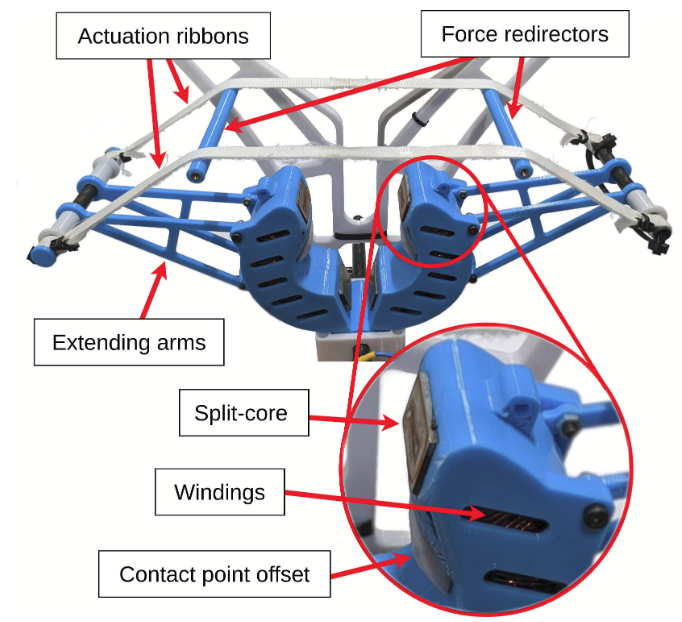
\includegraphics[width=\textwidth]{screenshots/clasp-1.png}
            \caption{Close-up side view of the perching device.}
            \label{fig:clasp:1}
        \end{subfigure}
        \hfill
        \begin{subfigure}[b]{0.45\textwidth}
            \centering
            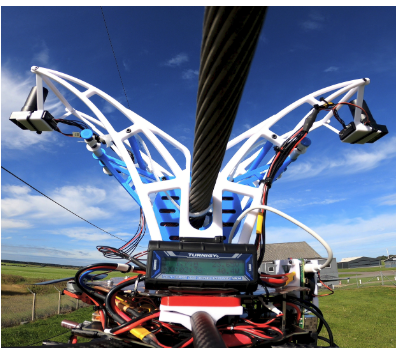
\includegraphics[width=\textwidth]{screenshots/clasp-2.png}
            \caption{Perching device and drone attached to a power line.}
            \label{fig:clasp:2}
        \end{subfigure}
    \end{subfigure}
    \caption{An example of a perching mechanism designed to attach to and charge from power lines. \ref{fig:clasp:1} shows
    a close up of the grasper and charging device, \ref{fig:clasp:2} shows the device and drone attached to a power line.
    Adapted from \cite{hoang_autonomous_2024}.}
    \label{fig:clasp}
\end{figure}

Hoang et al. demonstrated that their design was successful, with a field test lasting over two hours and containing 5 cycles of 
autonomously attaching to a power line, charging, then detaching and resuming flight \cite{hoang_autonomous_2024}.

The device designed by Kitchen et al. is similar to that designed by Hoang et al. The devices design is
illustrated in Fig. \ref{fig:kitchen-grasper}. It consists of a grasper and an inductive charging circuit, 
their grasper is actively actuated rather than passively. Kitchen et al. did not 
develop an autonomous detection and guidance system, and performed their testing in a laboratory environment by 
manually placing a drone on a simulated perch \cite{kitchen_design_2020}.


\begin{figure}[H]
    \centering
    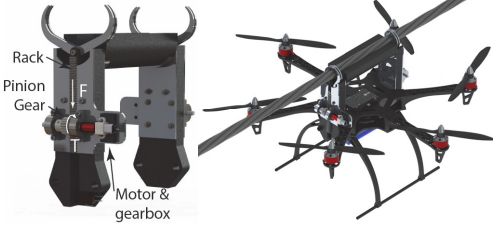
\includegraphics[width=\textwidth]{screenshots/kitchen-grasper.png}
    \caption{An example of an actively actuated perching mechanism designed to attach 
        to and charge from power lines. Adapted from \cite{kitchen_design_2020}.}
    \label{fig:kitchen-grasper}
\end{figure}


\subsubsection{Environmental Monitoring}

Forest canopies contain highly varied microclimates, which support diverse ecosystems and may provide additional resilience to climate change.
These systems are poorly understood, primarily due to the difficulty of observation and data collection. Often canopy cranes are used for
forest observation, however these are costly and not suitable for data collection over a broad area. 
They are also very large, and can themselves cause disruption to the system being studied \cite{nakamura_forests_2017}.
Other methods for tree canopy access include constructing towers, scaffolds, or aerial walkways through the tree canopy, 
though these methods are also inflexible, and they do not permit access to all levels of the canopy. Climbing can also 
allow researchers access to the canopy, but this requires training, poses a safety hazard, and only permits
access to lower levels where branches will support a humans weight \cite{parker_access_1992}.

Tropical forests are a primary target for global restoration and carbon sequestration efforts,
so increasing knowledge of these forests is critical for understanding how to protect them and the global climate \cite{mrema_ten_2020}.
Drones have potential as methods of collecting better data about forests. Being mobile, they can collect data over larger areas without the
need to construct replicated observation stations. The density of obstacles in a forest canopy can be a challenge for drones, but methods
to navigate similar environments have been proven \cite{mulgaonkar_robust_2018,tan_design_2017,liu_mini-drone_2023}. Two major problems
remain for using drones in ecological data collection: they are very loud and disruptive to wildlife being studied
\cite{jenni-eiermann_unmanned_2017,bennitt_terrestrial_2019}, and they have a short flight time due to their high power consumption.

Drones with perching features could allow sensors to be deployed in tree canopies without being limited by short flight time
or disturbing wildlife with loud noise. Kirchgeorg et al. designed a passive perching mechanism for this purpose, 
to attach a drone to tree branches using high-friction spines. Their design was intended to be resilient to
misalignment and avoid needing large open spaces for maneuvering and positioning \cite{kirchgeorg_hedgehog_2022}.
A number of other perching mechanisms targeting tree branch perching have been developed, such as the overhead grasping 
device designed bey Kirchgeorg et al. \cite{kirchgeorg_soft_2023} or the grapple device designed by Nguyen et al. \cite{nguyen_passively_2019}.

The possible uses for drone perching in ecological data collection may be overstated. A Michigan state affiliated researcher 
with experience in using drones for data collection shared that the main benefit of drones in their field is not the ability
to position sensors for long term collection, but their ability to sample a large area in a short amount of time. Additionally,
a drone and sensor payload often represents a large portion of an environmental researchers budget, and they are not likely
to be comfortable leaving it unattended in a tree \cite{_toto_cite_interview_}. Though it is worth considering that the 
forests of Michigan may provide a very different set of challenges for data collection than a tropical rainforest, and 
perching drones may still have use in specific environments.

Where perching an entire drone may be undesirable, a device such as that designed by Geckeler et al. could be used
to attach only a small and low-cost sensor payload, with the drone acting only as a delivery and retrieval mechanism.
Their design is passively actuated, using an elastic coil to wrap around a perch once the device is pressed against the
perch by a drone \cite{geckeler_bistable_2022}. 


\subsubsection{Networking}

Another application of drone perching is to establish temporary sensor networks using drone swarms. Seiber et al. propose using
swarms of drones equipped with air quality sensors to monitor the perimeter of hazardous gas plumes, such as might be 
released from a toxic material spill. This provides two benefits compared to manual data collection: removing humans
from identification of the plume boundaries reduces risk that humans will be exposed to toxins, and a network connected
drone swarm can provide lower latency than manual data collection \cite{seiber_tracking_2018}.

Seiber et al. propose a drone design that is constantly in flight, providing a visual cue to the perimeter of a plume
that first responders can use; since the drones are programmed to fly towards the outer edge of the gas cloud,
first responders simply look up to see where the drones currently are \cite{seiber_tracking_2018}. Liu et al. point out
that the short battery life of most drones is a limiting factor to this approach, and propose using perching drones for 
establishing sensor and communication networks. Using drones with perching abilities provides the benefit of quickly deploying
a network in hazardous or hard to reach areas, while extending mission time by shutting down flight systems once a perching 
location has been found \cite{liu_perching_2022}.


\subsection{Modes of Perching}

Meng et al. identify 3 primary modes of drone perching in their review \cite{meng_aerial_2022}. The modes identified are:
\begin{itemize}
    \item Grasping based perching mechanisms.
    \item Embedding based perching mechanisms.
    \item Attaching based perching mechanism.
\end{itemize}

\subsubsection{Grasping}

Grasping based mechanisms use attachments that can grip a perch with enough force to hold a drone stationary.
Often they are inspired by birds claws and are designed to allow a drone to sit on top of its perch. One benefit
of such a method is that the grasper can, if correctly designed, serve dual use as a perching device as well as
a grasper for carrying or manipulating objects \cite{meng_aerial_2022}.

One example of a grasping based mechanism is proposed by Chi et al., and shown in Fig. \ref{fig:claw}. It aims 
to imitate the biomechanics of bird legs. The design proves capable of holding a 2kg mass stationary on a perch, 
both in static testing and when dropped onto a perch \cite{chi_optimized_2014}.

\begin{figure}[H]
    \centering
    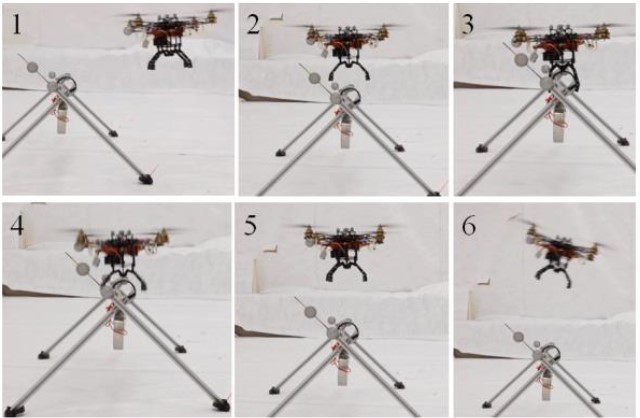
\includegraphics[width=\textwidth]{screenshots/claw.jpg}
    \caption{An example of a claw-like perching mechanism, where the drone lands on a perch and remains fixed by closing the claw. Adapted from \cite{chi_optimized_2014}.}
    \label{fig:claw}
\end{figure}

Though many grasping based perching mechanisms are inspired by avian biomechanics, some take a different approach and attach a drone to a perch from the bottom via a mechanical clasping mechanism.
The device proposed by Hoang et al. shown in Fig. \ref{fig:clasp}, which is intended for use in power line inspection, is such a device.
It uses ribbons to passively close an electromagnetic clasp once the drone has approached the appropriate position below a power line. 
Once closed, current harvested from the power line can be used to keep clasp closed as well as recharge the drone \cite{hoang_autonomous_2024}.

The device designed by Kominami et al., shown in Fig. \ref{fig:passive}, is another grasping type device that grasps a perch beneath the drone. 
A distinguishing feature of this design is that it is passively driven; the grasping force is provided by the weight of the drone on top of the grasper \cite{kominami_detection_2023}.

\begin{figure}[H]
    \centering
    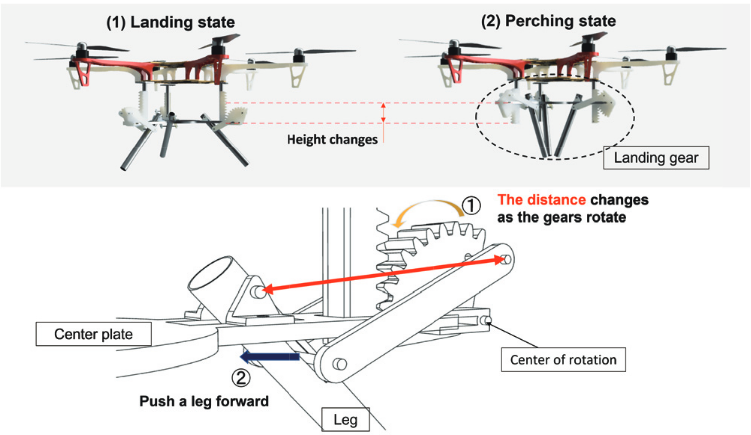
\includegraphics[width=\textwidth]{screenshots/passive.png}
    \caption{A passively actuated perching mechanism that uses the drones weight to provide the grasping force. Adapted from \cite{kominami_detection_2023}.}
    \label{fig:passive}
\end{figure}


\subsubsection{Embedding}

Embedding based perching mechanisms take advantage of the texture of a surface and spikes on the drone to attach the drone to the surface. 
This works similarly to how many insects climb surfaces, by using tiny spikes that grasp onto microscopic cracks or bumps on a surface. 
This method can allow drones to perch on vertical surfaces, though it is not universal to all surface types and 
can provide less stability than grasping based methods \cite{meng_aerial_2022}. 

Distinguishing between grasping and embedding mechanisms can be simply a matter of scale, as embedding mechanisms often operate like very small graspers.
Fig. \ref{fig:gripper} illustrates a device proposed by Roderick et al. which is designed to grip the bark of a tree \cite{roderick_bioinspired_2017}.
While it does not attach by grasping an actuator around the circumference of a tree like a typical grasping based device would, Fig. \ref{fig:gripper}
shows that it is still operating by grasping onto smaller scale features.

\begin{figure}[H]
    \centering
    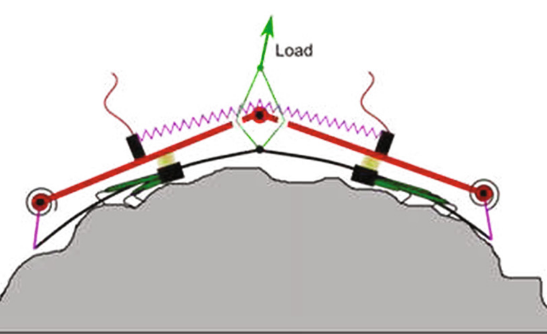
\includegraphics[width=\textwidth]{screenshots/bark gripper.png}
    \caption{Perching device designed to attach to the vertical side of a tree trunk. Adapted from \cite{roderick_bioinspired_2017}.}
    \label{fig:gripper}
\end{figure}


\subsubsection{Attaching}

Attaching based perching devices use adhesives, electromagnetics, electrostatics, or vacuum cups to attach a drone to a surface. Such methods
can work with both smooth and rough surfaces, unlike grasping or embedding methods, and can attach drones above, below, or to the side of a perch
object \cite{meng_aerial_2022}.

One example of such a device is shown in Fig. \ref{fig:electroadhesive}, designed by Gaule et al. It uses electrostatic adhesion to 
attach an insect inspired micro UAV to the underside of an object \cite{graule_perching_2016}.

\begin{figure}[H]
    \centering
    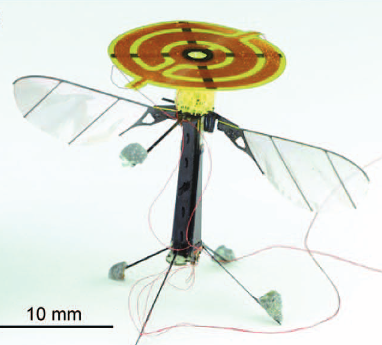
\includegraphics[width=\textwidth]{screenshots/electroadhesive.png}
    \caption{Example of an attaching based perching device that uses electrostatic adhesion. Adapted from \cite{graule_perching_2016}.}
    \label{fig:electroadhesive}
\end{figure}


\subsection{Perch Detection Methods}

Kominami et al. designed a perch detection method in conjunction with their passive grasping device shown in Fig. \ref{fig:passive}.
Their detection method is designed to detect long thin features that the grasper is designed to land on, such as signs and fences. 
Using a RealSense D405 RGB-D camera they implement the following image processing pipeline:

\begin{enumerate}
    \item RGB data is processed with a Hough transform to identify the top and bottom edge of a long thin board.
    \item The depth data is used to measure a depth profile of the board along a line perpendicular to the two edges.
    \item The shape of the depth profile is used to confirm the type of object detected.
    \item If a suitable object is confirmed, then the location of its top is returned.
\end{enumerate}

This method proved capable of identifying the board to perch on, though it suffers from being unable to identify a thin board when the drone is directly
above it \cite{kominami_detection_2023}.


An alternative detection method proposed by von Frankenberg and Nokleby uses a RANSAC method to detect cylindrical perches in a point cloud. They used a Microsoft
Kinect to acquire 3D point clouds and processed them using the following sequence:
\begin{enumerate}
    \item Downsample and crop point cloud.
    \item Identify possible lines with a RANSAC approach.
    \item Remove any lines that make an angle with the x-y plane steeper than $30^\circ$.
    \item Scan the length of each detected line and remove lines that have gaps where no points are detected.
    \item Scan the length of each detected line and remove lines that have points too close to the line, which indicates obstructions.
\end{enumerate}

The authors note that their algorithm was successfull in detecting a suitable test target, however it suffered from high computation time.
Using an Intel i7-4770 3.40 GHz 4 core processor their method was able to collect measurements at 10Hz with point clouds containing up to 5000
points, however processing time quickly increases as the number of point grows or if the point cloud becomes dominated by planar objects (their test 
scene shows only 2 ladders and a pair of pipes, all of which produce only thin line-like shapes in the point cloud). Additionally, the randomness
of the RANSAC method they use leads to the target object not being detected in every frame because its points were not selected in every frame \cite{von_frankenberg_detection_2020}.

\section{Methods}

\subsection{Conventions}

\subsubsection{Coordinate System} \label{sec:conv:coord}

Where coordinates are used, the cameras coordinate system is used. This means that, in an image frame from the camera's
perspective, the y-axis points up, the x-axis points left, and the z-axis extends into the depth dimension. 
This is illustrated in Fig. \ref{fig:coordinates}.

\begin{figure}[H]
    \centering
    \tdplotsetmaincoords{65}{115}
    \begin{tikzpicture}[tdplot_main_coords, scale=1.2, >=Stealth, line join=round] 
    %===================================================
    % Coordinate axes (camera frame: y up, z out of lens).
    % NOTE: to get y rendered as the vertical (up) axis with
    % these view angles, a *true* coordinate (X,Y,Z) is drawn
    % at the local pgf coordinate (X,Z,Y) throughout this
    % picture -- i.e. slot 2 <-> true z (depth), slot 3 <->
    % true y (height).
    %===================================================
    \draw[thick,-{Stealth[length=3mm]}] (0,0,0) -- (-1.5,0,0) node[above right]{$x$};
    \draw[thick,-{Stealth[length=3mm]}] (0,0,0) -- (0,0,1.5) node[above]{$y$};
    \draw[thick,-{Stealth[length=3mm]}] (0,0,0) -- (0,1.5,0) node[below right]{$z$};
    \filldraw[black] (0,0,0) circle (0.02);
    
    %===================================================
    % Vertical rod, parallel to the y axis, passing through
    % the z axis at some positive depth
    %===================================================
    \pgfmathsetmacro{\rodz}{2.6}
    \draw[ultra thick, black!60, line cap=round]
        (0,\rodz,-1.4) -- (0,\rodz,1.4);
    \filldraw[black!60] (0,\rodz,-1.4) circle (0.03);
    \filldraw[black!60] (0,\rodz, 1.4) circle (0.03);
    \node[anchor=west] at (0,\rodz,1.55) {Perch};
    
    %===================================================
    % Simple stereo camera, sitting on the negative z axis,
    % looking down the +z direction
    %===================================================
    \pgfmathsetmacro{\camz}{-1.8}
    
    % camera body (a flat box in the x-y plane at depth z = \camz)
    \draw[fill=black!75, draw=black]
        (-0.75,\camz,-0.3) -- (0.75,\camz,-0.3) --
        (0.75, \camz, 0.3) -- (-0.75, \camz, 0.3) -- cycle;
    
    % two lenses, offset along x (stereo baseline).
    % "circle" always draws in the flat, screen-facing canvas plane,
    % so it must be re-anchored into the camera body's own plane
    % (fixed local y = \camz, varying local x/z) via a canvas scope.
    \begin{scope}[canvas is xz plane at y=\camz]
        \filldraw[fill=black!40, draw=black] (-0.38,0) circle (0.2);
        \filldraw[fill=black!40, draw=black] ( 0.38,0) circle (0.2);
        \filldraw[fill=black]                (-0.38,0) circle (0.07);
        \filldraw[fill=black]                ( 0.38,0) circle (0.07);
    \end{scope}
    
    % dashed line showing the camera's viewing (+z) direction
    \draw[dashed, gray] (0,\camz,0) -- (0,0,0);
    
    \node[anchor=north] at (0,\camz,-0.45) {Stereo Camera};
    \end{tikzpicture}
    \caption{Illustration of coordinate conventions used in this thesis, where the z-axis extends
    outward from the cameras focal point and the y-axis extends vertically in the cameras frame.
    The illustration shows a test setup with the camera on the left and a test perch being detected
    on the right.}
    \label{fig:coordinates}
\end{figure}

\subsubsection{Measurements} \label{sec:conv:meas}

There are 3 position measurements relevant for the perch detection 
in this thesis:
\begin{itemize}
    \item Distance: $d$, distance along the z-axis between the camera and test object. Illustrated in Fig. \ref{fig:distance}
    \item Azimuth: $\alpha$, Angle between the y-axiz and the test object. Illustrated in Fig. \ref{fig:angles}
    \item Elevation: $\theta$, Angle between the x-y plane and the test object. Illustrated in Fig. \ref{fig:angles}
\end{itemize}

\begin{figure}[H]
    \centering
    \tdplotsetmaincoords{65}{115}
    \begin{tikzpicture}[tdplot_main_coords, scale=1.2, >=Stealth, line join=round] 
    %===================================================
    % Coordinate axes (camera frame: y up, z out of lens).
    % NOTE: to get y rendered as the vertical (up) axis with
    % these view angles, a *true* coordinate (X,Y,Z) is drawn
    % at the local pgf coordinate (X,Z,Y) throughout this
    % picture -- i.e. slot 2 <-> true z (depth), slot 3 <->
    % true y (height).
    %===================================================
    \draw[thick,-{Stealth[length=3mm]}] (0,0,0) -- (-1.5,0,0) node[above right]{$x$};
    \draw[thick,-{Stealth[length=3mm]}] (0,0,0) -- (0,0,1.5) node[above]{$y$};
    \draw[thick,-{Stealth[length=3mm]}] (0,0,0) -- (0,1.5,0) node[below right]{$z$};
    \filldraw[black] (0,0,0) circle (0.02);
    
    %===================================================
    % Vertical rod, parallel to the y axis, passing through
    % the z axis at some positive depth
    %===================================================
    \pgfmathsetmacro{\rodz}{2.6}
    \draw[ultra thick, black!60, line cap=round]
        (0,\rodz,-1.4) -- (0,\rodz,1.4);
    \filldraw[black!60] (0,\rodz,-1.4) circle (0.03);
    \filldraw[black!60] (0,\rodz, 1.4) circle (0.03);
    \node[anchor=west] at (0,\rodz,1.55) {Perch};
    
    %===================================================
    % Simple stereo camera, sitting on the negative z axis,
    % looking down the +z direction
    %===================================================
    \pgfmathsetmacro{\camz}{-1.8}
    
    % camera body (a flat box in the x-y plane at depth z = \camz)
    \draw[fill=black!75, draw=black]
        (-0.75,\camz,-0.3) -- (0.75,\camz,-0.3) --
        (0.75, \camz, 0.3) -- (-0.75, \camz, 0.3) -- cycle;
    
    % two lenses, offset along x (stereo baseline).
    % "circle" always draws in the flat, screen-facing canvas plane,
    % so it must be re-anchored into the camera body's own plane
    % (fixed local y = \camz, varying local x/z) via a canvas scope.
    \begin{scope}[canvas is xz plane at y=\camz]
        \filldraw[fill=black!40, draw=black] (-0.38,0) circle (0.2);
        \filldraw[fill=black!40, draw=black] ( 0.38,0) circle (0.2);
        \filldraw[fill=black]                (-0.38,0) circle (0.07);
        \filldraw[fill=black]                ( 0.38,0) circle (0.07);
    \end{scope}
    
    % dashed line showing the camera's viewing (+z) direction
    \draw[dashed, gray] (0,\camz,0) -- (0,0,0);

    % dashed line showing the distance measurement
    \draw[dashed, red] (0,\camz,-1) -- (0,\rodz,-1) node[midway,below,red]{d};
    
    \node[anchor=north] at (0,\camz,-0.45) {Stereo Camera};
    \end{tikzpicture}
    \caption{Illustration of the distance measurement from the stereo camera to the perch.}
    \label{fig:distance}
\end{figure}

\begin{figure}[H]
    \centering
    \tdplotsetmaincoords{65}{115}
    \begin{tikzpicture}[tdplot_main_coords, scale=1.2, >=Stealth, line join=round] 
    %===================================================
    % Coordinate axes (camera frame: y up, z out of lens).
    % NOTE: to get y rendered as the vertical (up) axis with
    % these view angles, a *true* coordinate (X,Y,Z) is drawn
    % at the local pgf coordinate (X,Z,Y) throughout this
    % picture -- i.e. slot 2 <-> true z (depth), slot 3 <->
    % true y (height).
    %===================================================
    \draw[thick,-{Stealth[length=3mm]}] (0,0,0) -- (-1.5,0,0) node[above right]{$x$};
    \draw[thick,-{Stealth[length=3mm]}] (0,0,0) -- (0,0,1.5) node[above]{$y$};
    \draw[thick,-{Stealth[length=3mm]}] (0,0,0) -- (0,1.5,0) node[below right]{$z$};
    \filldraw[black] (0,0,0) circle (0.02);

    \coordinate (O) at (0,0,0);
    \tdplotsetcoord{P}{3}{25}{135}    
    \draw[dashed, red] (O) -- (Pxz);
    \draw[dashed, red] (O) -- (Pz);
    
    %===================================================
    % Vertical rod, parallel to the y axis, passing through
    % the z axis at some positive depth
    %===================================================
    \pgfmathsetmacro{\rodz}{0}
    \pgfmathsetmacro{\rodl}{3}
    \tdplotsetrotatedcoords{135}{25}{0}
    \begin{scope}[tdplot_rotated_coords]
        \draw[ultra thick, black!60, line cap=round]
            (0,\rodz,-\rodl) -- (0,\rodz,\rodl);
        \filldraw[black!60] (0,\rodz,-\rodl) circle (0.03);
        \filldraw[black!60] (0,\rodz, \rodl) circle (0.03);
        \node[anchor=west] at (0,\rodz,\rodl+0.15) {Perch};
    \end{scope}

    \pic[draw=red, text=red, "$\theta$", angle radius=2cm, angle eccentricity=1.3] {angle = P--O--Pxz};
    \pic[draw=red, text=red, "$\alpha$", angle radius=2.5cm, angle eccentricity=1.3] {angle = Pxz--O--Pz};

    \end{tikzpicture}
    \caption{Illustration of the angle measurements of a perch's orientation: $\alpha$, the angle between the perch
        and the y-axis, and $\theta$, the angle between the perch and the x-y plane.}
    \label{fig:angles}
\end{figure}

\subsubsection{Point Cloud Rendering} \label{sec:conv:ptcld}

Point cloud data shown in this thesis contains data about 3D points, as 
well as lines that were detected by the perch detection algorithm. 
To display multiple detected lines in point cloud data, points that are assigned
to a line are shown with a color, while other background is shown in black and white. 
Point cloud data is displayed in one of two ways:
\begin{itemize}
    \item As a screenshot of point cloud data displayed in 3D, as shown in Fig. \ref{fig:ptcld-display}
    \item Overlaid on the image captured by the left camera, from which the point cloud was taken, 
        as shown in Fig. \ref{fig:ptcld-overlay}
\end{itemize}

Note that in both displays, the different colors used have no specific meaning; the only intent of the different 
colors is to visually distinguish clusters of points that belong to different lines.

\begin{figure}[H]
    \centering
    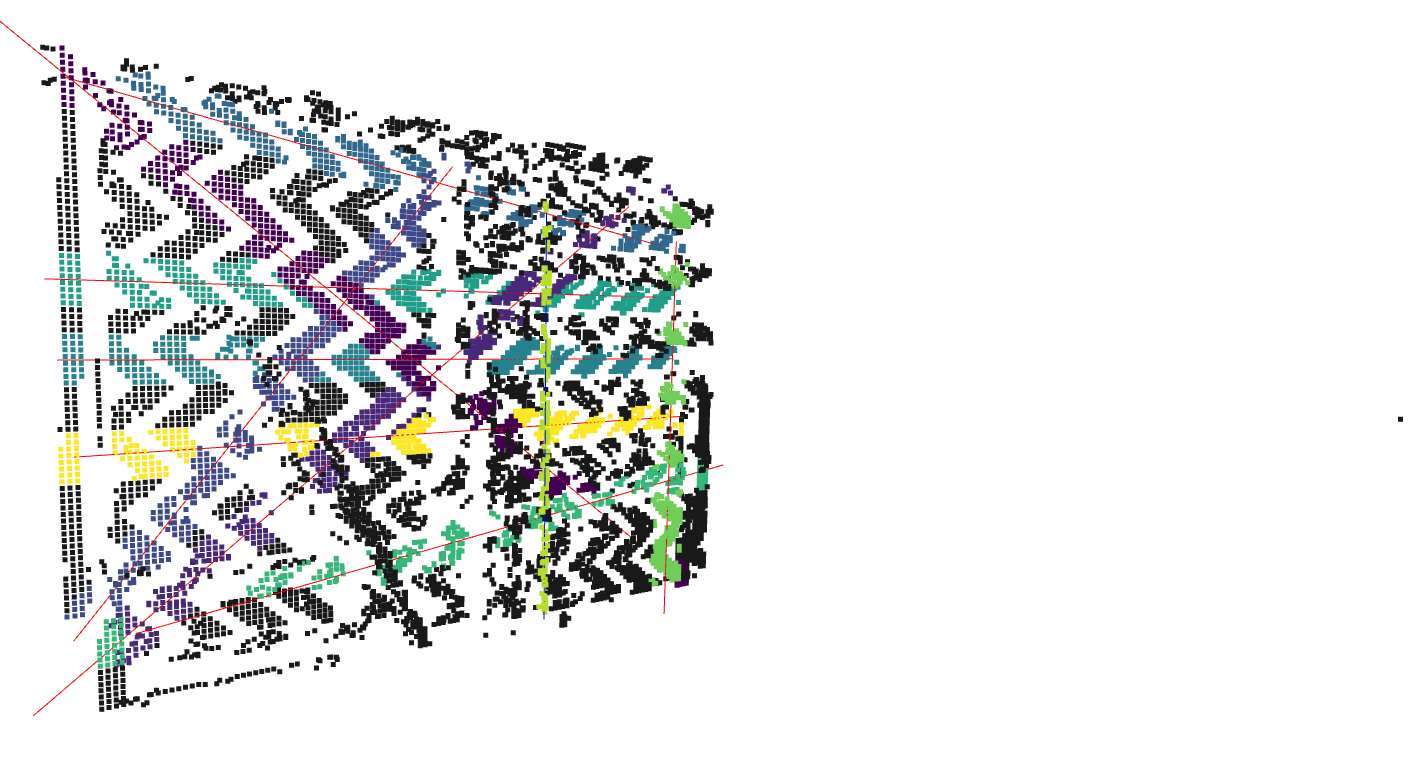
\includegraphics[width=\textwidth]{sections/discussion/zigzag-ptcld-2-obj.png}
    \caption{
        Example of a point cloud display. For each line, the points that belong to it are shown by highlighting
        those points a different color. The lines are also drawn in the point cloud to precisely show their detected
        size and orientation. Only one line is selected as the correct candidate object, and it is drawn in blue. The
        rejected candidate lines are drawn in red. In this example the selected candidate is near the center of the image,
        vertical, and the points belonging to it are shown in lime green. Since it was selected as the correct object,
        its precise size and orientation are shown with a thin blue line passing through the cluster of lime green points.
    }
    \label{fig:ptcld-display}
\end{figure}


\begin{figure}[H]
    \centering
    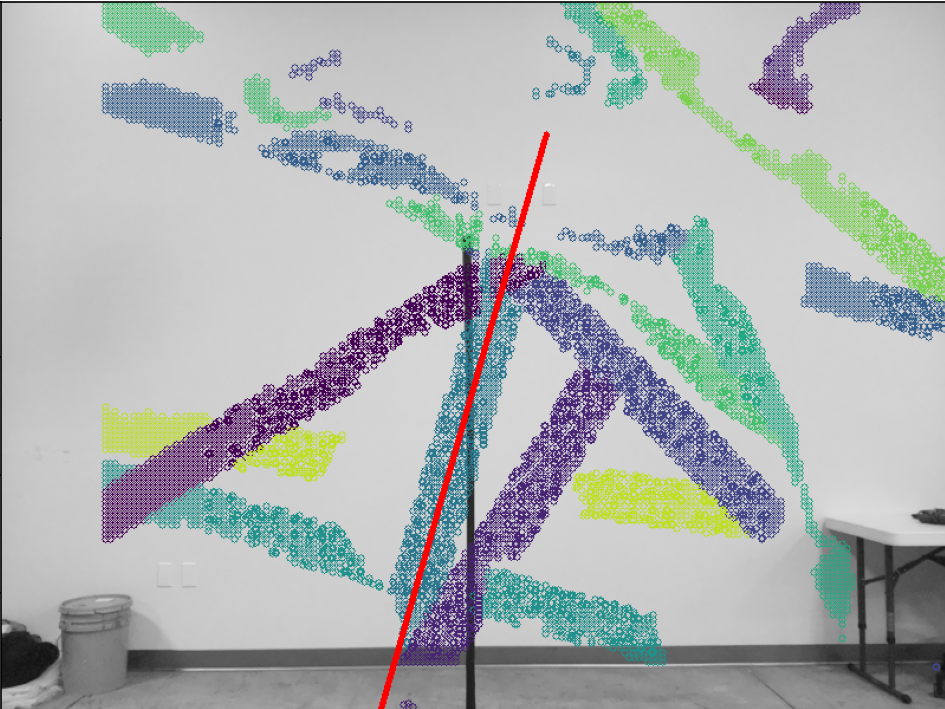
\includegraphics[width=\textwidth]{sections/methods/label_bad_3.png}
    \caption{
        Example of a point cloud overlaid on a grayscale image. Each detected line is shown by projecting the points 
        belonging to it into the 2D image coordinates and highlighting those points a unique color. The line selected
        as the correct object as a solid red line drawn through it showing its precise position and orientation. This
        sample includes many lines that do not correspond to real objects, due to poorly generated disparity data over the 
        textureless backgorund.
    }
    \label{fig:ptcld-overlay}
\end{figure}
\subsection{Grasper Design}

\subsubsection{Latch Mechanism}

The chosen design for the grasper consists of a rotating clasp, driven by a servo motor. A rendering of the design
is shown in Fig. \ref{fig:clasp-design}, and the OpenSCAD source used to create it can be found in appendix \ref{app:grasper-scad}.
The \texttt{BOSL2} library \cite{belfryscad_bosl2_nodate} was used to create the gear components.

\begin{figure}[H]
    \centering
    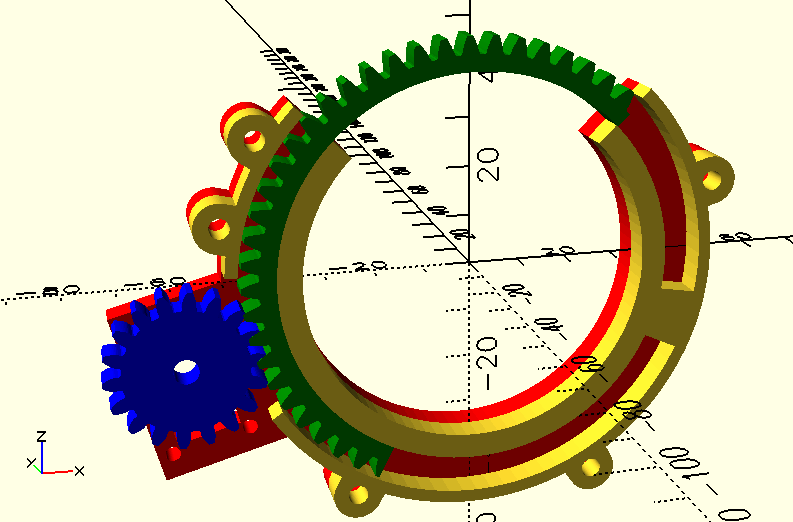
\includegraphics[width=\textwidth]{sections/methods/grasper-render.png}
    \caption{Rendering of the proposed grasping device. The backplate shown in red is meant to hold 
    a servo, which drives the gear shown in blue. The green, toothed semicircle is driven by the blue gear to
    open and close the grasper, and bears the weight of the device and drone once closed over a perch. The
    yellow part supports and guides the green latch. Note that in the real device there is a third plate closing 
    the front of the device, but it is not shown here so that the gear and latch mechanism are visible.}
    \label{fig:clasp-design}
\end{figure}

The device used here has an inner radius of 35mm, which results in it being able to accept a perch of up to 
50mm diameter. The outer radius of the device is 50mm. The latch component (green object in Fig. \ref{fig:clasp-design})
has a radial width of 7.4mm.

\subsubsection{Controller}

A Raspberry Pi Compute Module 4 was used to control the servos on the grasper device. To avoid 
complicating the design with limit switches to detect open and closed states, an Adafuit 
ADS1015 analog-digital converter was used to measure the current drawn by each servo.
The current measurement is used to detect when the servo has stalled, indicating 
that the limits of travel are reached and the latch has either fully opened or closed.

The schematic of the servo control module can be seen in appendix \ref{app:schematics},
Fig. \ref{fig:clasp-ctl}. The schematic showing the compute module and its interface to the
servo controller can be seen in appendix \ref{app:schematics},
Fig. \ref{fig:cpu-module}.


\subsection{Grasper Verification}

\subsubsection{Holding Capacity}

The specifications of popular commercial drones were assessed to determine common weights of drones,
to determine weight that this drone might need to support.
Table \ref{tab:drone-weights} shows the assessed models and their weights.

\begin{table}[H]
    \centering
    \caption{Specified Weight of Various Commercial Drones}
    \begin{tabular}{| c || c |}
        \hline
        {Make \& Model} & Weight (g) \\
        \hline
        DJI Mavic Pro & 734 \\
        DJI Mavic 3 Pro & 958 \\
        DJI Mavic 3 Enterprise & 920 \\
        DJI Mavic Mini & 249 \\
        Parrot ANAFI USA & 500 \\
        FLIR SIRAS & 3100 \\
        Autel EVO Max 4T & 1640 \\
        DJI Matrice 30 & 3770 \\
        \hline
    \end{tabular}
    \label{tab:drone-weights}
\end{table}

There appear to be a few classes of drones represented:
\begin{itemize}
    \item Sub 500g lightweight drones
    \item Sub 1kg medium drones
    \item Heavy weight 1.5 kg + drones
\end{itemize}

This device was designed to hold a drone of up to 500g, plus 31.58 N
of dynamic load, for a total static load of 3.72 kg.

The dynamic load is to allow for force introduced by motion of the perch, such as a swaying tree branch.
Assuming that the drone is perched in a tree and subject to sinusoidal motion, its maximum acceleration is estimated at $63.17 m/s^2$ 
based on data provided by Kamimura et al. (0.4 m max displacement with a frequency of 2 Hz) \cite{kamimura_energy_2024}.  
The referenced study did use only Japanese Cedar, which may not
be representative of all trees. However, similar data for other species could not be found.

The first reason for targeting the lowest weight group is that the low weight is far more
manageable for the device to hold. The other reasons are cost and risk. The medium and heavy drones tend to be significantly 
more expensive, and are used to carry higher quality cameras. Leaving a drone perched in a tree or other location leaves
it exposed to risk of damage, which makes using a larger drone for this particularly unappealing to the drone's owner.

The achieved holding capacity of the device was achieved with the following test process:
\begin{enumerate}
    \item The grasper was closed around a test perch, suspended above the ground.
    \item A bag was attached to the underside of the grasper, close to the center of its baseplate in the x-y plane.
    \item Weights were added to the bag incrementally, with a 10-minute period between each addition.
    \item Once the device breaks before the 10-minute period has expired after the most recent addition, the holding capacity
        is determined to be the load weight at the previous successful weight addition.
\end{enumerate}

To avoid damaging the electronic components when the device failed, all except the servos were removed for the duration of this test. 
The device is capable of remaining attached without power to the servos, and the weight of the removed electronics was removed from the
final weight at the end of the test. The results are summarized in Section \ref{sec:results:capacity}


\subsubsection{Weight}

Table \ref{tab:payload} shows rated payload for various drones, which were used 
The rated payload was calculated as the rated maximum total takeoff weight minus the drones specified weight. 
The DJI Mavic products had no maximum takeoff weight aside from the products weight, so no maximum payload is listed for them. 

\begin{table}[H]
    \centering
    \caption{Rated Payload of Various Commercial Drones}
    \begin{tabular}{| c || c |}
        \hline
        {Make \& Model} & Payload (g) \\
        \hline
        DJI Mavic Pro & None Rated \\
        DJI Mavic 3 Pro & None Rated \\
        DJI Mavic 3 Enterprise & 130 \\
        DJI Mavic Mini & None Rated \\
        Parrot ANAFI USA & 144 \\
        FLIR SIRAS & 3100 \\
        Autel EVO Max 4T & 379 \\
        DJI Matrice 30 & 299 \\
        \hline
    \end{tabular}
    \label{tab:payload}
\end{table}

In the sub 500g category, only the Parrot ANAFI has a rated payload. This will be assumed as a reasonable estimate for the
payload capacity of similarly sized drones. In order to leave some margin for safety, and possible additional task-specific
modifications, this devices weight shall be no more than 33\% of that capacity, or 47.5g. This target weight will also 
provide improvements over similar existing designs \cite{chi_optimized_2014,nguyen_passively_2019}.

The overall weight and weight of individual components of the device were measured and recorded in table \ref{tab:weights}.

\subsubsection{Repeatability}

To verify that the proposed design can open and close reliably, the opening and closing process was manually 
repeated 30 times. Each time after closing the grasper or opening it again, the device was 
visually inspected to ensure that:
\begin{itemize}
    \item The latch had not become stuck on any other part of the device, causing stall detection to trigger
        prematurely and prevent successful opening or closing.
    \item The latch had not failed to engage with the servo, preventing it from moving.
\end{itemize}

If opening or closing was not successful, then that test was marked as a failure, and the specific reason recorded.
The success rate and failure causes are shown in Section \ref{sec:results:repeatability}.
\subsection{Perch Detection Software Design}

The image processing software used to validate the perch detection concept was implemented in C++ and executed on a Raspberry Pi Compute Module 4. The graph in figure 
\ref{fig:sw-flow} provides a high-level illustration of the steps in the image processing pipeline and how data flows between them.

\begin{figure}[H]
    \centering
    \digraph[width=\textwidth]{swflow}{
        rankdir=TB;
        lc [label="Left Camera Frame Acqusision" shape=box];
        rc [label="Right Camera Frame Acqusision" shape=box];
        ls [label="Left Stereo Block Matching" shape=box];
        rs [label="Right Stereo Block Matching" shape=box];
        f [label="Weighted Least Squares Filtering" shape=box];
        pc [label="Point Cloud Projection and Downsampling" shape=box];
        ht [label="3D Hough Transform" shape=box];
        s [label="Best Candidate Selection" shape=box];

        lc -> ls [label="Left Side Image"];
        lc -> rs [label="Left Side Image"];
        lc -> f [label="Guide For Inpainting"];
        rc -> ls [label="Right Side Image"];
        rc -> rs [label="Right Side Image"];
        ls -> f [label="Left-To-Right Disparity"];
        rs -> f [label="Right-To-Left Disparity"];
        f -> pc [label="Filtered Disparity and Confidence Map"];
        pc -> ht [label="Down-Sampled Point Cloud"];
        ht -> s [label="Position, Orientation, and Dimensions of Candidate Lines"];        
    }
    \caption{Diagram of the dataflow for the proposed image processing pipeline, starting from image aquisition on the top
        to generation of coordinates for the detected perch on the bottom.}
    \label{fig:sw-flow}
\end{figure}



\subsection{Stereo Camera Calibration}

A camera calibration script was creates using the functions available in OpenCV \cite{bradski_opencv_2000}. The script can be read in appendix \ref{app:cal-code}.
285 total calibration image pairs were captured. The calibration pattern used was an 8 marker by 11 marker ChArUco board with 20mm checkers and 15mm markers, and a 4x4 AruCo dictionary.

To perform individual camera intrinsic and distortion parameter calibrations, each image was loaded and the pattern corners were detected and mached to the expected board layout.
Any image in which fewer than 10 corner points were detected was discarded, as low point counts can result in bad calibration parameters. For accepted images, the identified calibration
pattern corner locations in the image coordinates are saved, as well as the estimated position and orientation of the calibration board. The accepted points were then used to calculate 
an initial estimate of the cameras intrinsic matrix and distotion coefficients. The calibration at this point is still low quality, so an iterative refinement is now applied. For each image
that was not rejected, the calibration pattern points are projected into image coordinates using the saved position and orientation estimates of the calibration board. Then the error between these 
projected points and the positions of the previously detected points in that image were calculated. Once these errors were calculated for all images, any point in an image that had a reprojection error 
greater than 3 standard deviations of the reprojection error for all points in all images was discarded, under the assumption that this high error was due to a bad detection of that corner. If any image 
contained less then 10 valid points after removing points with high error, the entire image was discarded. This process was repeated until either one of the following termination criteria was met:

\begin{itemize}
    \item The change in standard deviation of the reprojection errors for all points in all images was less than $1e-9$.
    \item The iteration limit of $5$ was reached.
\end{itemize}


The stereo translation and rotation parameter calibration process followed a similar design, however in the initial filtering and later iterative remove, only points 
that were valid in both images were retained (ChArUco patterns use QR-like codes that allow points to be identified uniquely across different images or in partial occlusions).
So if calibration point A was detected in the left image but not in the right image, or if it was detected in both but then was removed from the left point set due to too high 
reprojection error, then it was not used in either. Image pairs that had less than 10 valid points in either left or right image were rejected from both sets. 

After following this process for each individual camera, and then for the stereo combination, 26 images were retained as valid for the left camera, 17 for the right camera, and 
10 images retained for the stereo combination. A visual inspection of the reprojection errors and detected corner locations was performed to confirm that:

\begin{itemize}
    \item The errors were approximately zero-mean.
    \item The errors had approximately the same distribution in the x and y directions.
    \item The detected marker locations covered most of the camera frame, to avoid overfitting to non-symetrical lens defects on one portion of the image. 
\end{itemize}

Figures \ref{fig:cal-left}, \ref{fig:cal-right}, and \ref{fig:cal-stereo} show the visualizations used to perform this inspection of calibration results.

\begin{figure}[H]
    \centering
    \begin{subfigure}[b]{0.45\textwidth}
        \centering
        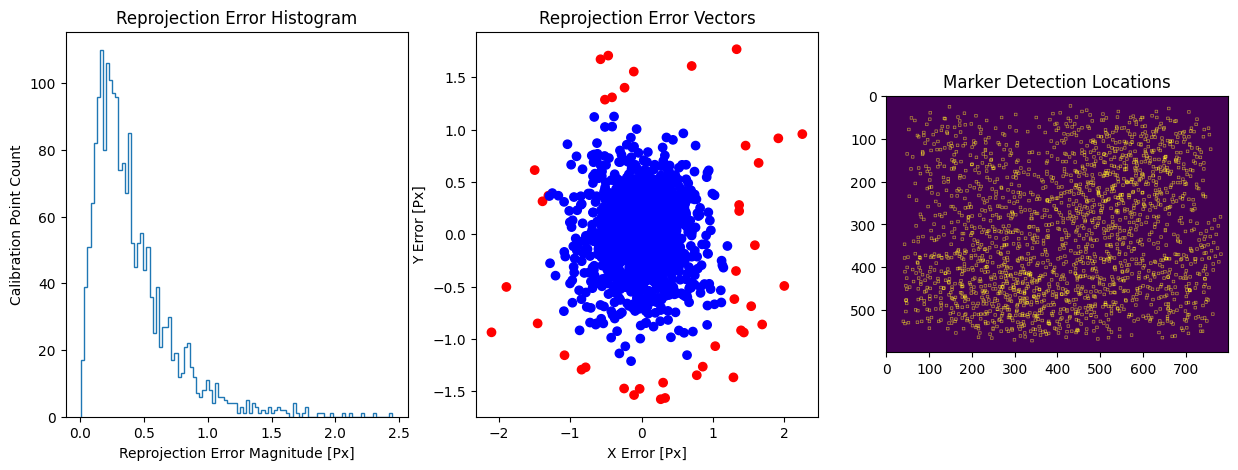
\includegraphics[width=\textwidth]{sections/methods/left-cal-pre.png}
        \caption{Before removing outliers.}
        \label{fig:cal-left-1}
    \end{subfigure}
    \vfill
    \begin{subfigure}[b]{0.45\textwidth}
        \centering
        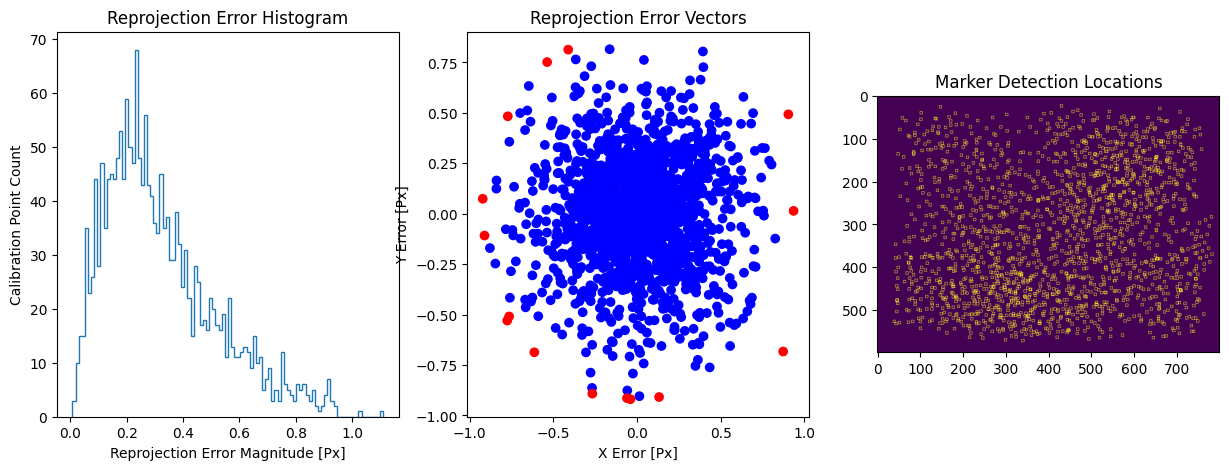
\includegraphics[width=\textwidth]{sections/methods/left-cal-post.png}
        \caption{After removing outliers.}
        \label{fig:cal-left-2}
    \end{subfigure}
    \caption{Calibration visualizations for the left camera, before (\ref{fig:cal-left-1}) and after (\ref{fig:cal-left-2}) iterative outlier removal.}
    \label{fig:cal-left}
\end{figure}

\begin{figure}[H]
    \centering
    \begin{subfigure}[b]{0.45\textwidth}
        \centering
        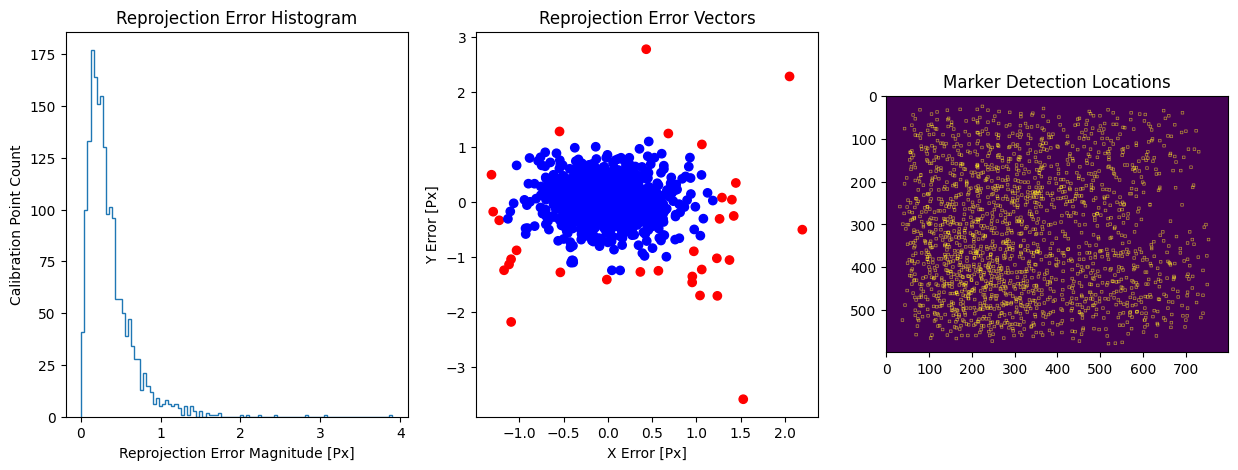
\includegraphics[width=\textwidth]{sections/methods/right-cal-pre.png}
        \caption{Before removing outliers.}
        \label{fig:cal-right-1}
    \end{subfigure}
    \vfill
    \begin{subfigure}[b]{0.45\textwidth}
        \centering
        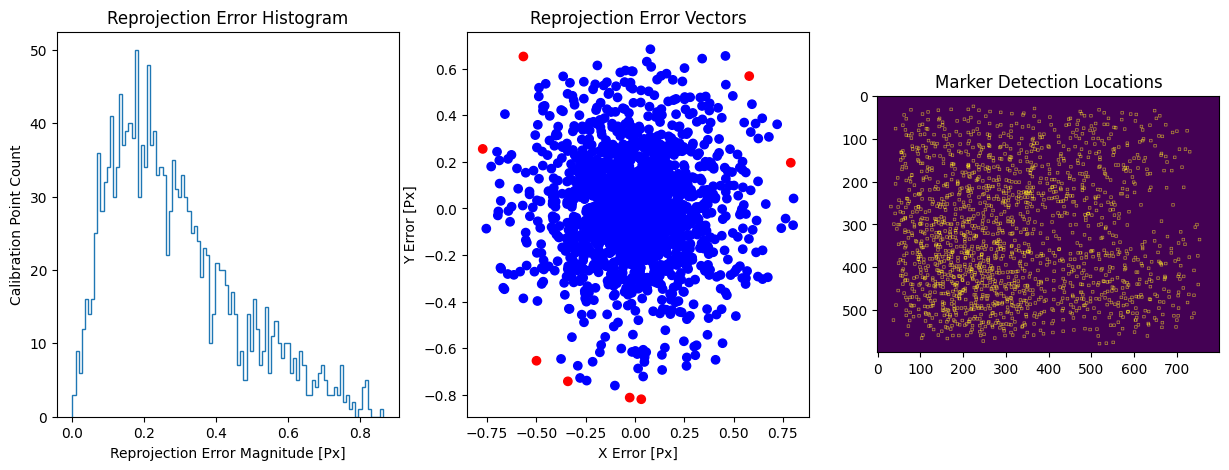
\includegraphics[width=\textwidth]{sections/methods/right-cal-post.png}
        \caption{After removing outliers.}
        \label{fig:cal-right-2}
    \end{subfigure}
    \caption{Calibration visualizations for the right camera, before (\ref{fig:cal-right-1}) and after (\ref{fig:cal-right-2}) iterative outlier removal.}
    \label{fig:cal-right}
\end{figure}

\begin{figure}[H]
    \centering
    \begin{subfigure}[b]{0.45\textwidth}
        \centering
        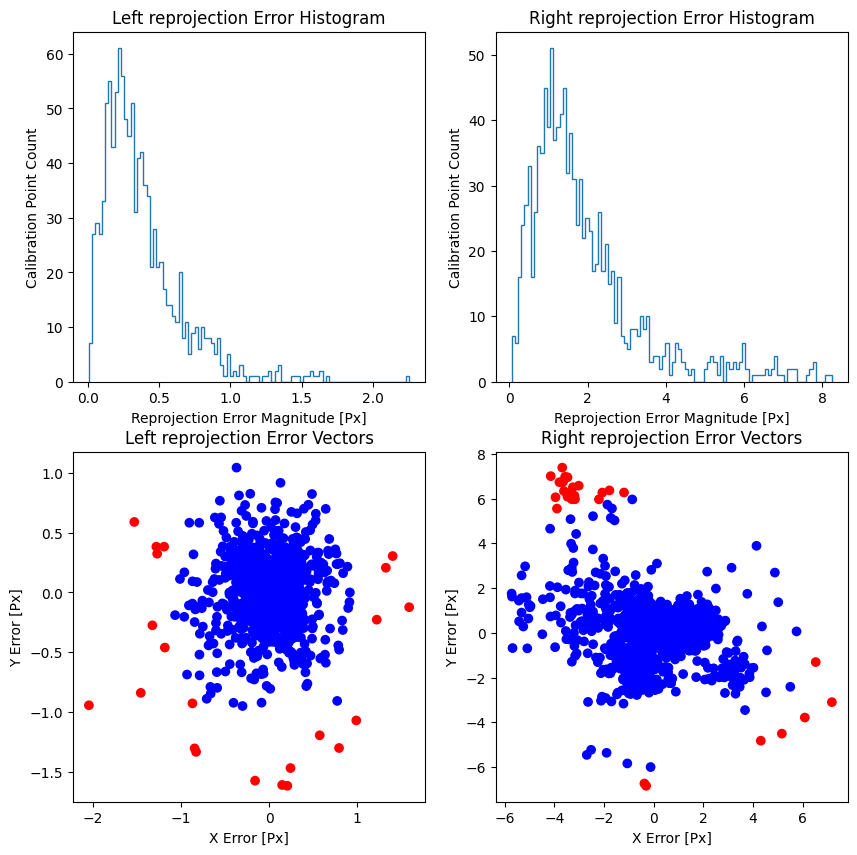
\includegraphics[width=\textwidth]{sections/methods/stereo-cal-pre.png}
        \caption{Before removing outliers.}
        \label{fig:cal-stereo-1}
    \end{subfigure}
    \vfill
    \begin{subfigure}[b]{0.45\textwidth}
        \centering
        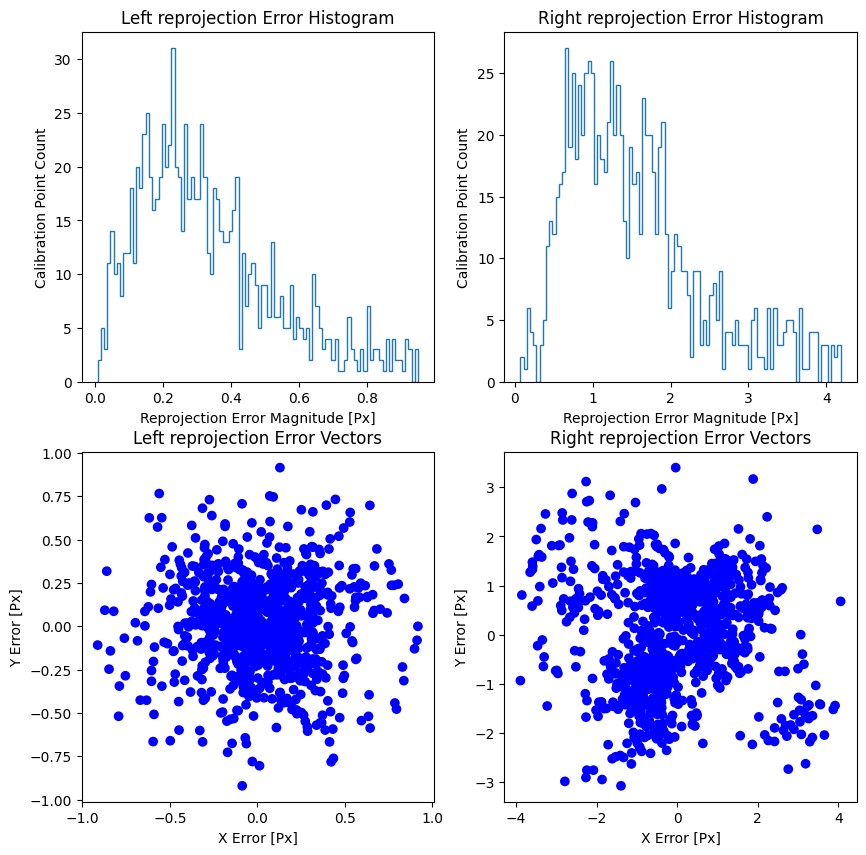
\includegraphics[width=\textwidth]{sections/methods/stereo-cal-post.png}
        \caption{After removing outliers.}
        \label{fig:cal-stereo-2}
    \end{subfigure}
    \caption{Calibration visualizations for the stereo pair, before (\ref{fig:cal-stereo-1}) and after (\ref{fig:cal-stereo-2}) iterative outlier removal.}
    \label{fig:cal-stereo}
\end{figure}

\subsection{Perch Detection Validation Data Collection}

To first test the detection methods performance under the most controlled conditions, the device was placed facing a flat white wall, indoors,
with only one object (a gray, 15mm diameter PVC pipe) in the frame. The object was placed at a distance $d = 1000mm$ from the camera, at an azimuth angle (angle between
object and cameras y axis) $\theta = 0^\circ$ and elevation angle (angle between the cameras x-y plane and the object) $\phi = 0^\circ$.

The image processing program was started by the script found in appendix \ref{app:data-coll-code}. Once the output of the program indicated that at least one
candidate line had been detected, the program was run for 2 minutes. The script monitored the detection results via serial terminal and saved the position, 
orientation, and dimensions of the detected object each time a new update was produced by the detection program. At each new update the script also triggered the
program to save a binary file containing both left and right images, the calculated disparity and confidence map, the filtered point cloud, and information about the 
identified line candidates with labels for all points in the point cloud that belong to a line canditate.

This test was performed for the following combinations of object poses. All angles were measured to be within $5^\circ$ of the target value using the "Clinometer" Android app,
and the distances measured within $5mm$ via tape measure.

\begin{itemize}
    \item $d = 5000mm$, $\theta = 0^\circ$, $\phi = 0^\circ$
    \item $d = 1000mm$, $\theta = 0^\circ$, $\phi = 0^\circ$
    \item $d = 2000mm$, $\theta = 0^\circ$, $\phi = 0^\circ$
\end{itemize}

These three trials were then repeated with the object in front of a zig-zag background pattern. The motivation for this test is to compare the success rate in best and worst case conditions; the 
flat white wall tends to be the most difficult case for the detection process due to the lack of features for stereo matching to use. The zig-zag background serves as a more optimistic performance test.

A review of initial results showed that the performance against the white wall background was poor. A possible method to improve this is to threshold the left image into light and dark regions, and
only include points whose color falls in the dark region in the point cloud. This assumes that the target object will always be darker than the background. For a perching device facing upward towards
open sky or tree canopies, this assumption may hold true. To implement this the "Weighted Least Squares Filtering" in figure \ref{fig:sw-flow} was modified to include the following algorithm:

\begin{enumerate}
    \item A Gaussian blur with a 5x5 kernel is applied to the left camera image.
    \item A threshold value is determined for the blurred image via Otsu's method.
    \item For each pixel with an intensity greater than the threshold value, the corresponding disparity value is set to -1. 
        Negative disparity values result in invalid points whcih get filtered out in the "Point Cloud Projection and Downsampling" step of figure \ref{fig:sw-flow}
\end{enumerate}

This was tested again with both white and zig-zag backgrounds. The tests with added threshold filtering were performed by processing saved data from the first test trials through the
image processing pipeline rather than collecting new data. The script in appendix \ref{app:retest-code} was used to process this new test data.

Table \ref{tab:vision-test-cases} shows all test cases that were perform.

\begin{table}[H]
    \centering
    \caption{List of test scenarios for which data was collected.}
    \label{tab:vision-test-cases}
    \begin{tabular}{c|cc}
        Case Number & Background Type & Threshold Based Filter \\
        \hline
        1 & White & Off  \\
        2 & Zig-Zag & Off \\
        3 & White & On \\
        4 & Zig-Zag & On
    \end{tabular}
\end{table}

\subsection{Perch Detection Validation Data Analysis}

The first analysis performed on the detection data was determining how often the device correctly detected the object. This 
was done using the binary files saved in the data collection process alongside the script in appendix \ref{app:label-code}.
This script displays the left camera image from each file and overlays the selected line candidate, alongside colored dots 
indicating all points that are part of a candidate line. This allows the user to accept an image as a valid detection, or
reject it if something appears to have gone wrong in the processing. The script then saves a JSON file containing the 
overall sucess rate as a percentage of the files that were accepted by the user, as well as a boolean flag for each file
indicating if the user accepted or rejected it.

When labelling samples as valid or in valid, the follwing two criteria were used for determining if a detection was valid:
\begin{itemize}
    \item The line drawn to show the detected object must intersect somewhere with the real object.
    \item The line drawn to show the detected object must be approximately $10^\circ$ or less away from parallel to the real object.
\end{itemize}


\section{Results}

\subsection{Grasper Verification}

\subsubsection{Holding Capacity} \label{sec:results:capacity}

Table \ref{tab:weight-inc} shows the weight increments added to the 


\subsubsection{Weight}

\begin{table}[H]
    \centering
    \caption{Weights of Grasper Components}
    \label{tab:weights}
    \begin{tabular}{
        |>{\raggedright\arraybackslash}m{0.33\textwidth}|>{\raggedright\arraybackslash}m{0.33\textwidth}||
        >{\raggedright\arraybackslash}m{0.15\textwidth}|}
        \hline
        Component & Photo & Weight [g]\\
        \hline
        Base Plate and Clasp Mounts & ??? & ??? \\
        Grasper One & ??? & ??? \\
        Grasper Two & ??? & ??? \\
        CPU, Cameras, and Other Electronics & ??? & ??? \\
        \hline
        Total Weight & ??? & ??? \\
        \hline
    \end{tabular}
\end{table}


\subsubsection{Repeatability} \label{sec:results:repeatability}


\subsection{Perch Detection Success Rate}

For each test trial in table \ref{tab:vision-test-cases}, table \ref{tab:success-rates} shows
the percentage of samples in which the object was correctly detected. Table \ref{tab:success-rates-dist}
shows the same data, but with success rates reported for each distance between camera and object that 
was tested.

\begin{table}[H]
    \centering
    \caption{Detection success rate for each background in table \ref{tab:vision-test-cases}.}
    \label{tab:success-rates}
    \begin{tabular}{|c||c|}
        \hline
        Background & Success Rate [\%] \\
        \hline
        White & 100.0  \\
        Zigzag & 83.3 \\
        Checker & 31.7 \\
        \hline
    \end{tabular}
\end{table}

\begin{table}[H]
    \centering
    \caption{Detection success rate for each background and distance in table \ref{tab:vision-test-cases}}
    \label{tab:success-rates-dist}
    \begin{tabular}{|c|c||c|}
        \hline
        Background & Distance to Object [mm] & Success Rate [\%] \\
        \hline
        White & 500 & 100.0 \\
        White & 1000 & 100.0 \\
        White & 2000 & 100.0 \\
        Zigzag & 500 & 100.0 \\
        Zigzag & 1000 & 100.0 \\
        Zigzag & 2000 & 50.0 \\
        Checker & 500 & 90.0 \\
        Checker & 1000 & 5.0 \\
        Checker & 2000 & 0.0 \\
        \hline
    \end{tabular}
\end{table}


\subsection{Multi Object Success Rate}

Table \ref{tab:success-rates-multi} shows the success rate for each background when a second object was added behind the intended target.
Table \ref{tab:success-rates-multi-dist} shows the success rates for the same tests but split out by individual distances.

\begin{table}[H]
    \centering
    \caption{Detection success rate for each background tested with two objects.}
    \label{tab:success-rates-multi}
    \begin{tabular}{|c||c|}
        \hline
        Background & Success Rate [\%] \\
        \hline
        White & 100.0  \\
        Zigzag & 90.0 \\
        Checker & 0.0 \\
        \hline
    \end{tabular}
\end{table}

\begin{table}[H]
    \centering
    \caption{Detection success rate for each background and distance tested with two objects.}
    \label{tab:success-rates-dist-multi}
    \begin{tabular}{|c|c||c|}
        \hline
        Background & Distance to Object [mm] & Success Rate [\%] \\
        \hline
        White & 1000 & 100.0 \\
        White & 2000 & 100.0 \\
        Zigzag & 1000 & 100.0 \\
        Zigzag & 2000 & 80.0 \\
        Checker & 1000 & 0.0 \\
        Checker & 2000 & 0.0 \\
        \hline
    \end{tabular}
\end{table}


\section{Discussion}

\subsection{Perch Detection Success Rate}

The results show that the proposed image processing method has potential, though performance is dependent on the background.
Both patterned backgrounds performed worse than the plain white wall, with the checkered pattern performing extremely poorly (not
even a 50\% success rate), and the zigzag background showing a much smaller performance reduction compared to the white wall than 
for the checkered background.

The reason for the difference between the success rate for checkered and zigzag background patterns is not immediately obvious. 
Inspecting the point cloud data for each reveals that the problem most likely lies in how the background pattern is interacting 
with the \texttt{StereoSGBM} block matcher. Fig. \ref{fig:pattern-compare} shows the differences in stereo camera data for two samples
from each background pattern. It shows that the checkered pattern produces a region of erroneous high disparity, which prevents the 
line detection algorithms from correctly selecting the test object. Further experimentation would be needed to determine exactly 
why that is happening, one possibility is that the checker pattern is too small compared to the block size or disparity range
that \texttt{StereoSGBM} was configured to use, leading to incorrect block matches.

\begin{figure}[H]
    \centering
    % Generated from "C:\\Users\\wyatt\\Documents\\GVSU\\Thesis\\august_test_data\\idc_sept_5\\blanket\\pvc_2000_0_0_0_bin_5"
    \begin{subfigure}[b]{\textwidth}        
        \begin{subfigure}[b]{0.32\textwidth}
            \centering
            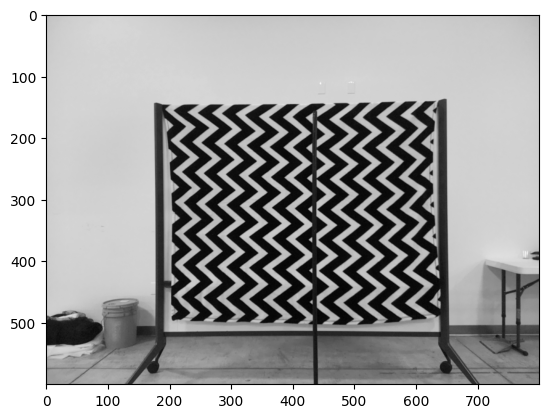
\includegraphics[width=\textwidth]{sections/discussion/zigzag-left-failure.png}
            \caption{Left camera image with zigzag background.}
            \label{fig:pattern-compare:zigzag:img}
        \end{subfigure}
        \hfill
        \begin{subfigure}[b]{0.32\textwidth}
            \centering
            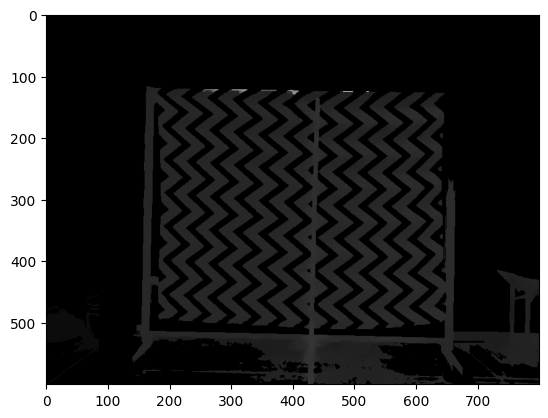
\includegraphics[width=\textwidth]{sections/discussion/zigzag-disp-failure.png}
            \caption{Disparity map calculated from \ref{fig:pattern-compare:zigzag:img} and the corresponding right image.}
            \label{fig:pattern-compare:zigzag:disp}
        \end{subfigure}
        \hfill
        \begin{subfigure}[b]{0.32\textwidth}
            \centering
            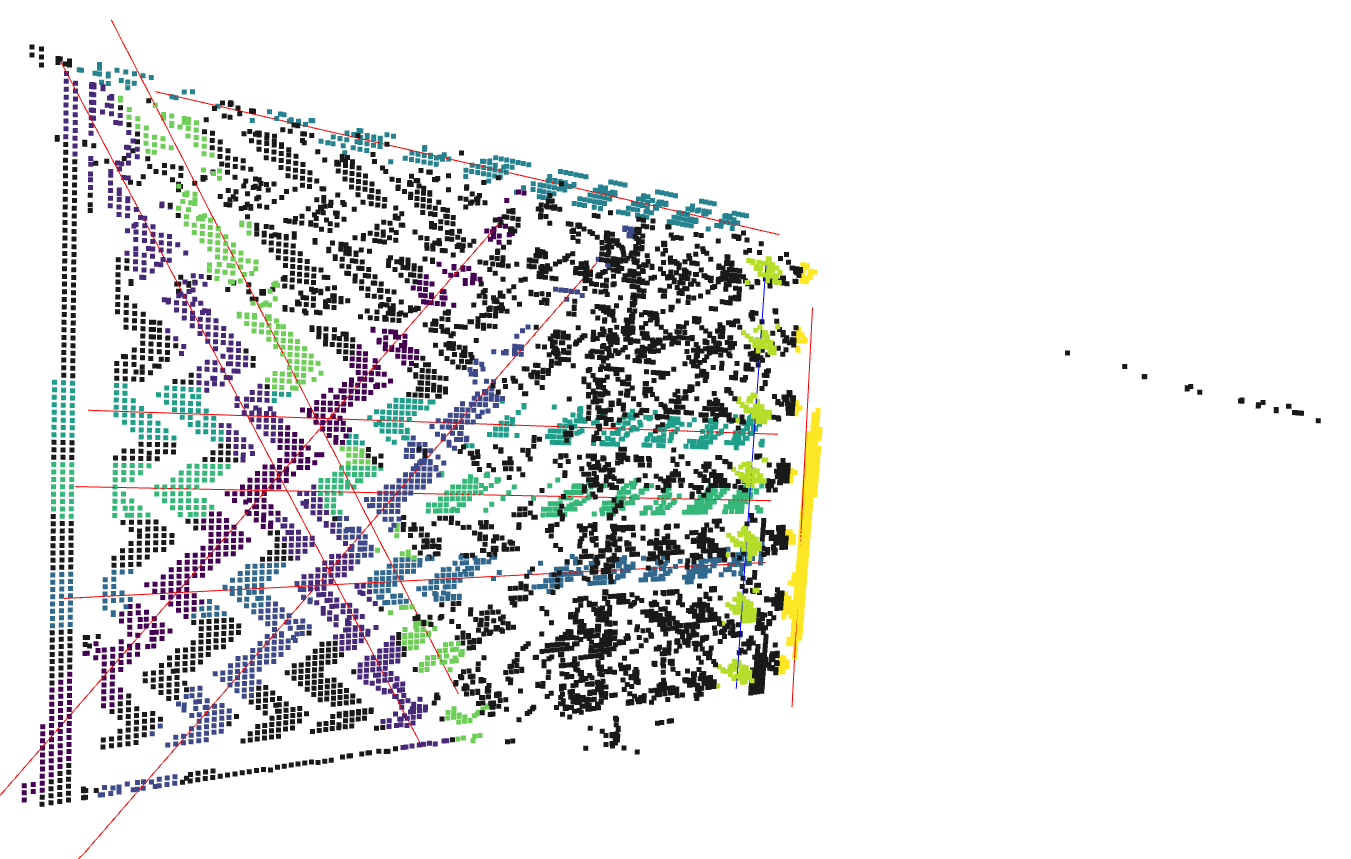
\includegraphics[width=\textwidth]{sections/discussion/zigzag-ptcld-failure.png}
            \caption{Point cloud produced from the disparity data in \ref{fig:pattern-compare:zigzag:disp}.}
            \label{fig:pattern-compare:zigzag:ptcld}
        \end{subfigure}
    \end{subfigure}
    \vfill
    \begin{subfigure}[b]{\textwidth}
        % Generated from "C:\\Users\\wyatt\\Documents\\GVSU\\Thesis\\august_test_data\\idc_sept_5\\cloth\\pvc_2000_0_0_0_bin_18"
        \begin{subfigure}[b]{0.32\textwidth}
            \centering
            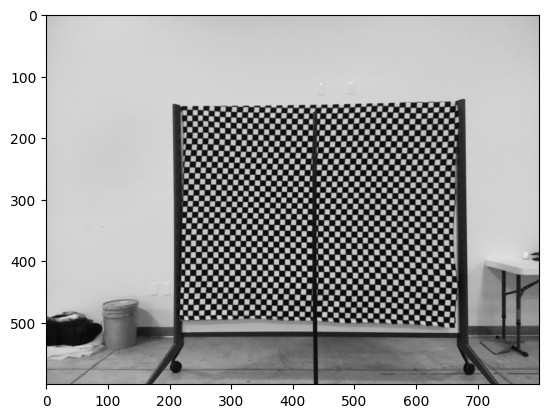
\includegraphics[width=\textwidth]{sections/discussion/check-left-failure.png}
            \caption{Left camera image with checkered background.}
            \label{fig:pattern-compare:check:img}
        \end{subfigure}
        \hfill
        \begin{subfigure}[b]{0.32\textwidth}
            \centering
            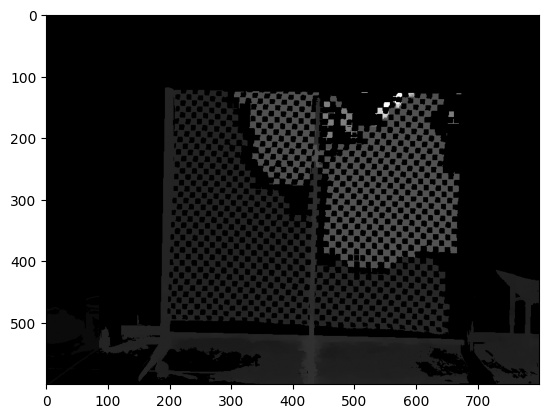
\includegraphics[width=\textwidth]{sections/discussion/check-disp-failure.png}
            \caption{Disparity map calculated from \ref{fig:pattern-compare:check:img} and the corresponding right image.}
            \label{fig:pattern-compare:check:disp}
        \end{subfigure}
        \hfill
        \begin{subfigure}[b]{0.32\textwidth}
            \centering
            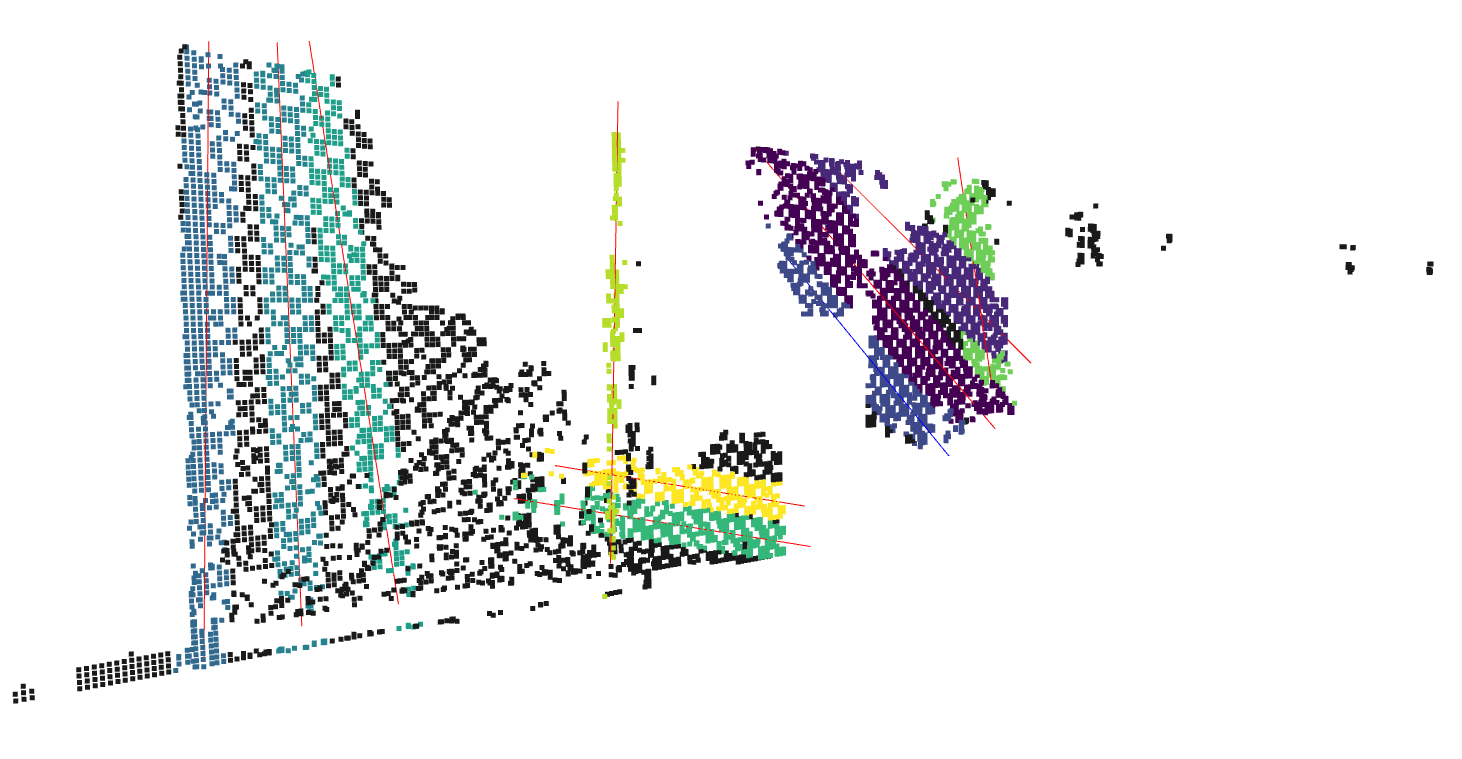
\includegraphics[width=\textwidth]{sections/discussion/check-ptcld-failure.png}
            \caption{Point cloud produced from the disparity data in \ref{fig:pattern-compare:check:disp}.}
            \label{fig:pattern-compare:check:ptcld}
        \end{subfigure}
    \end{subfigure}
    \caption{Comparison of sample data with the zigzag background and the checkered background. In both of the cases shown the object
        was not successfully detected. Note the region of high disparity in the upper right corner of the backdrop shown in \ref{fig:pattern-compare:check:disp},
        which is not seen in \ref{fig:pattern-compare:zigzag:disp}.}
    \label{fig:pattern-compare}
\end{figure}

The failures with the zigzag background do not appear to be a result of incorrect disparity data like the checkered background failures. 
Fig. \ref{fig:zigzag-fail-2} and \ref{fig:zigzag-fail-3} show sample data from two more failure cases with the zigzag background. Neither
Fig. \ref{fig:zigzag-fail-2:disp} nor \ref{fig:zigzag-fail-3:disp} show erroneous disparity artifacts such as seen in Fig. \ref{fig:pattern-compare:check:disp}.
Instead, the failures seem to be related to the Hough line detection. Fig. \ref{fig:zigzag-fail-2:ptcld-front} and \ref{fig:zigzag-fail-3:ptcld-front} 
show that the test object was not even identified as a target line (as it is shown in black and has no line drawn through it). This suggests that
the line did not meet the minimum vote threshold, or it had few enough votes that there were 10 higher voted incorrect lines.
Fig. \ref{fig:zigzag-fail-2:ptcld-side} and \ref{fig:zigzag-fail-3:ptcld-side} show that the test object was split up somewhat in 
the z axis, which may explain why its vote count was low. Lowering the minimum Hough vote threshold or raising the maximum number
of lines could help with this, though could also increase false detections due to poor quality background depth data.


\begin{figure}[H]
    \centering
    % Generated from "C:\\Users\\wyatt\\Documents\\GVSU\\Thesis\\august_test_data\\idc_sept_5\\blanket\\pvc_2000_0_0_0_bin_18"
    \begin{subfigure}[b]{\textwidth}
        \begin{subfigure}[b]{0.45\textwidth}
            \centering
            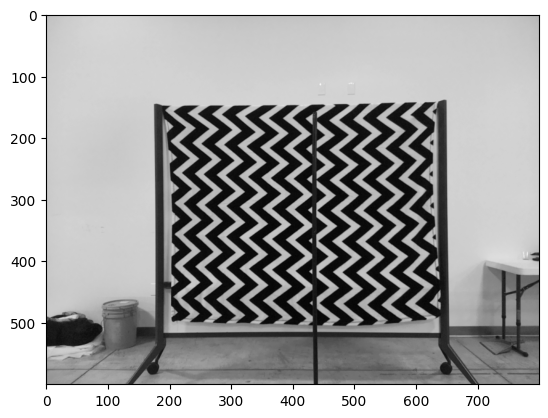
\includegraphics[width=\textwidth]{sections/discussion/zigzag-left-failure-2.png}
            \caption{Left camera image with the zigzag background pattern.}
            \label{fig:zigzag-fail-2:img}
        \end{subfigure}
        \hfill
        \begin{subfigure}[b]{0.45\textwidth}
            \centering
            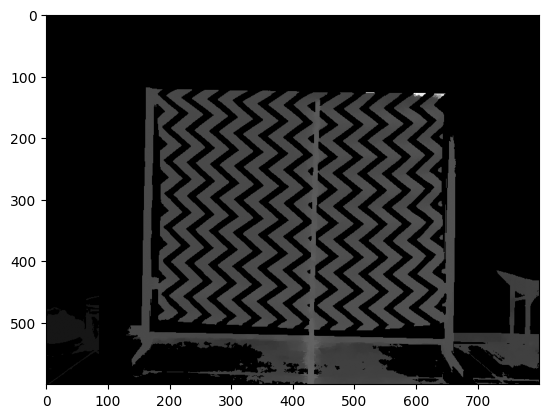
\includegraphics[width=\textwidth]{sections/discussion/zigzag-disp-failure-2.png}
            \caption{Disparity map produced from \ref{fig:zigzag-fail-2:img} and the corresponding right image.}
            \label{fig:zigzag-fail-2:disp}
        \end{subfigure}
    \end{subfigure}
    \vfill
    \begin{subfigure}[b]{\textwidth}
        \begin{subfigure}[b]{0.45\textwidth}
            \centering
            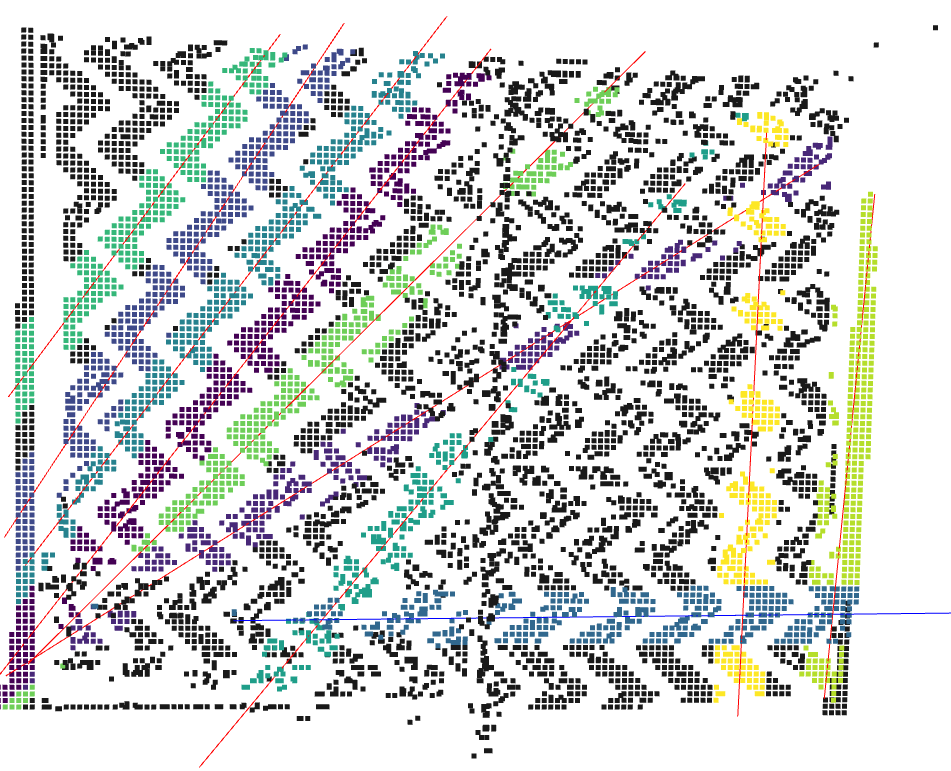
\includegraphics[width=\textwidth]{sections/discussion/zigzag-ptcld-failure-2-front.png}
            \caption{Front view of the point cloud produced from the disparity data in \ref{fig:zigzag-fail-2:disp}.}
            \label{fig:zigzag-fail-2:ptcld-front}
        \end{subfigure}
        \hfill
        \begin{subfigure}[b]{0.45\textwidth}
            \centering
            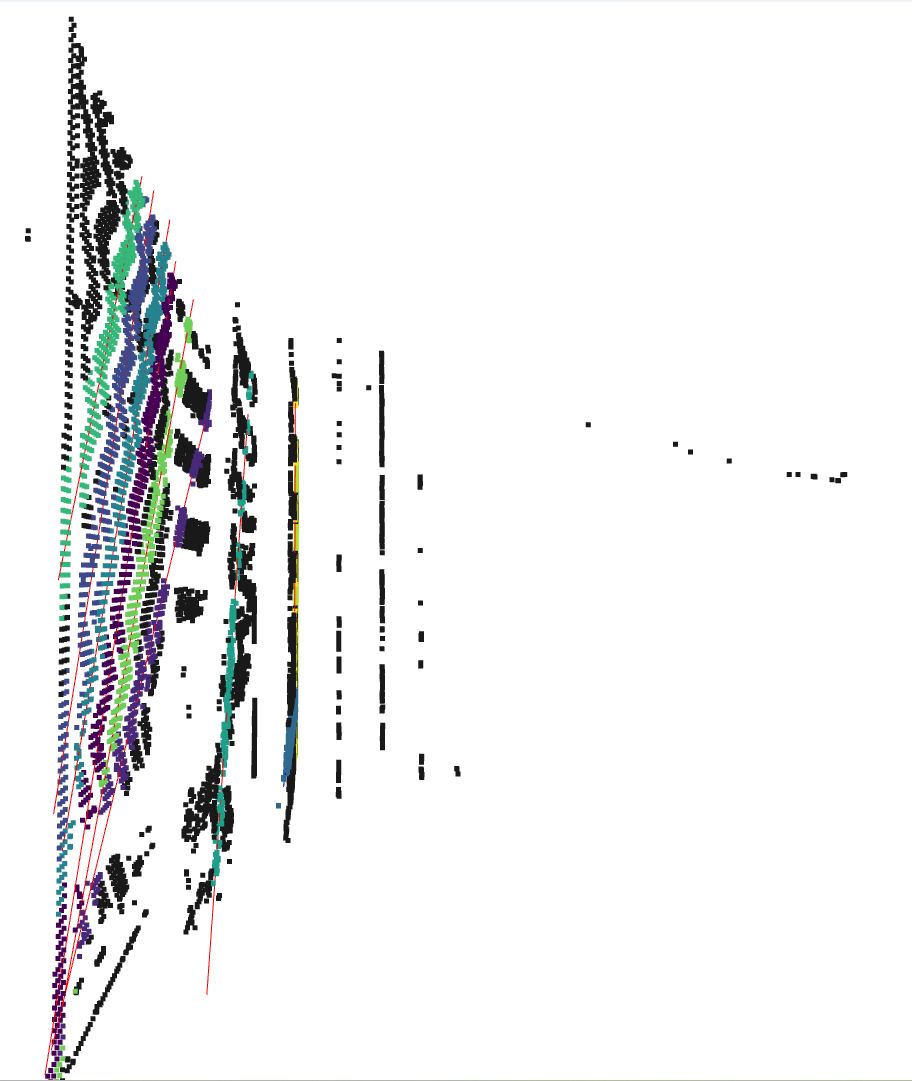
\includegraphics[width=\textwidth]{sections/discussion/zigzag-ptcld-failure-2-side.png}
            \caption{Side view of the same point cloud shown in \ref{fig:zigzag-fail-2:ptcld-front}.}
            \label{fig:zigzag-fail-2:ptcld-side}
        \end{subfigure}
    \end{subfigure}
    \caption{Sample failure case with the zigzag background. Note that the point cloud in \ref{fig:zigzag-fail-2:ptcld-front} and
    \ref{fig:zigzag-fail-2:ptcld-side} shows the test object was not identified as a candidate line.}
    \label{fig:zigzag-fail-2}
\end{figure}


\begin{figure}[H]
    \centering
    % Generated from "C:\\Users\\wyatt\\Documents\\GVSU\\Thesis\\august_test_data\\idc_sept_5\\blanket\\pvc_2000_0_0_0_bin_7"
    \begin{subfigure}[b]{\textwidth}
        \begin{subfigure}[b]{0.45\textwidth}
            \centering
            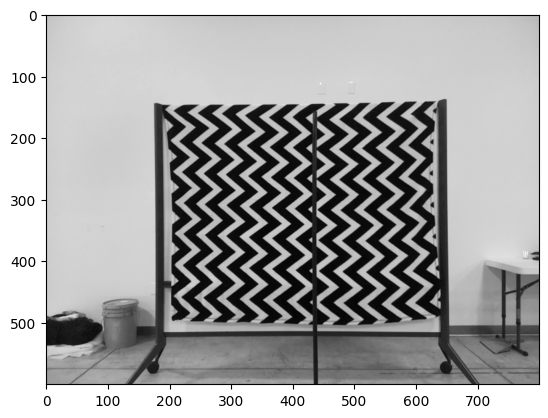
\includegraphics[width=\textwidth]{sections/discussion/zigzag-left-failure-3.png}
            \caption{Left camera image with the zigzag background pattern.}
            \label{fig:zigzag-fail-3:img}
        \end{subfigure}
        \hfill
        \begin{subfigure}[b]{0.45\textwidth}
            \centering
            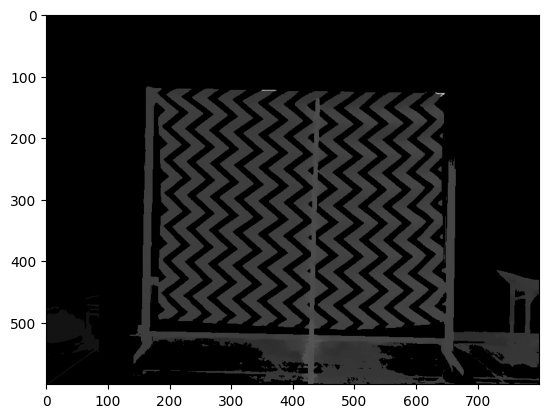
\includegraphics[width=\textwidth]{sections/discussion/zigzag-disp-failure-3.png}
            \caption{Disparity map produced from \ref{fig:zigzag-fail-3:img} and the corresponding right image.}
            \label{fig:zigzag-fail-3:disp}
        \end{subfigure}
    \end{subfigure}
    \vfill
    \begin{subfigure}[b]{\textwidth}
        \begin{subfigure}[b]{0.45\textwidth}
            \centering
            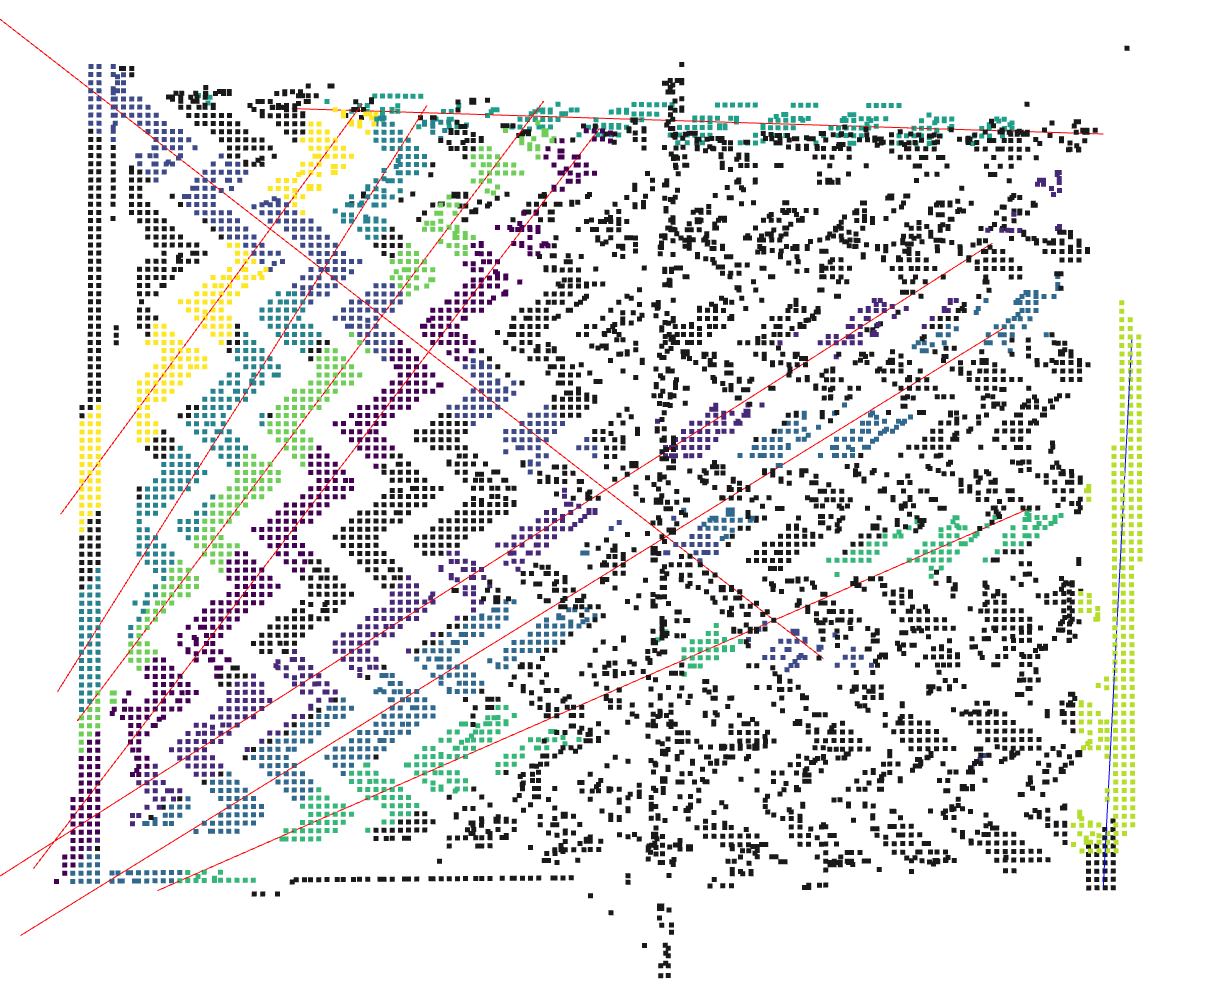
\includegraphics[width=\textwidth]{sections/discussion/zigzag-ptcld-failure-3-front.png}
            \caption{Front view of the point cloud produced from the disparity data in \ref{fig:zigzag-fail-3:disp}.}
            \label{fig:zigzag-fail-3:ptcld-front}
        \end{subfigure}
        \hfill
        \begin{subfigure}[b]{0.45\textwidth}
            \centering
            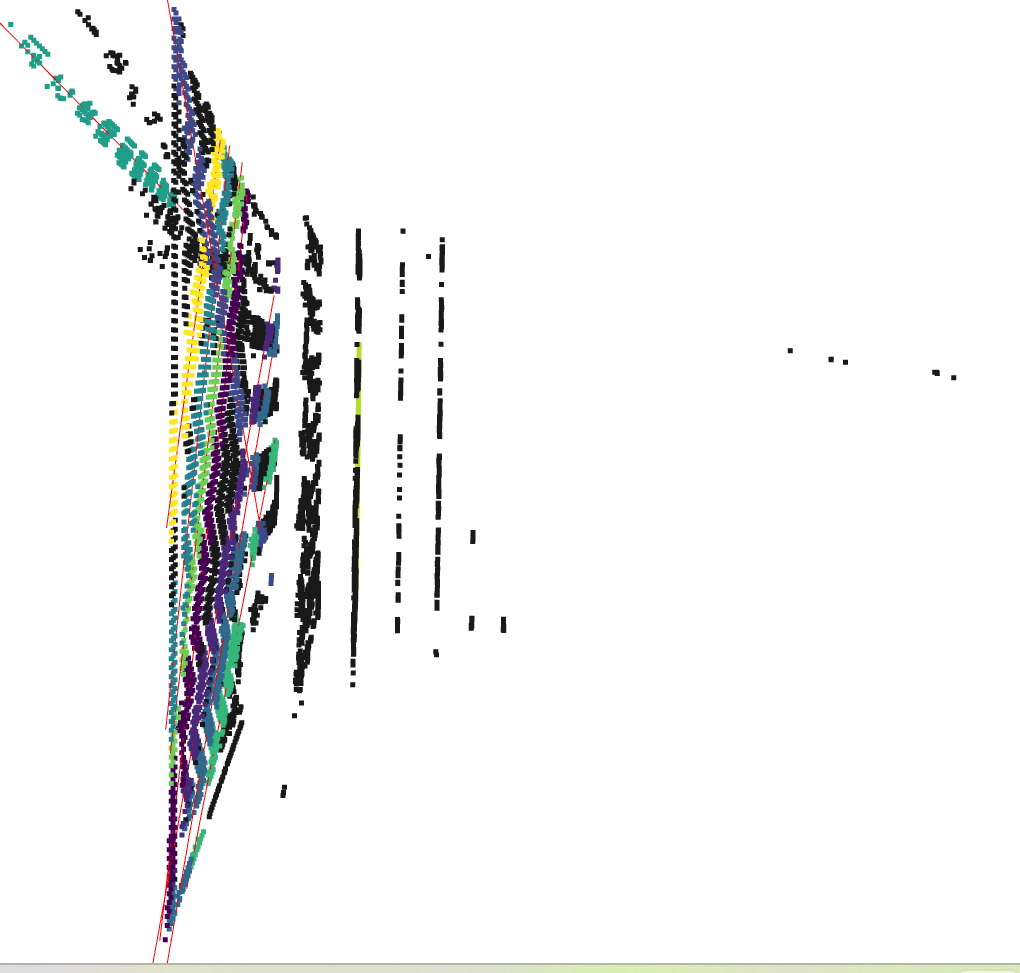
\includegraphics[width=\textwidth]{sections/discussion/zigzag-ptcld-failure-3-side.png}
            \caption{Side view of the same point cloud shown in \ref{fig:zigzag-fail-3:ptcld-front}.}
            \label{fig:zigzag-fail-3:ptcld-side}
        \end{subfigure}
    \end{subfigure}
    \caption{Sample failure case with the zigzag background. Note that the point cloud in \ref{fig:zigzag-fail-3:ptcld-front} and
    \ref{fig:zigzag-fail-3:ptcld-side} shows the test object was not identified as a candidate line.}
    \label{fig:zigzag-fail-3}
\end{figure}


\subsection{Multiple Object Success Rate}

Table \ref{tab:success-rates-dist-multi} shows that, against the flat white background, adding a second object behind the first did not
impact the success rate. The checkered background does not show a significant difference (p > 0.05 via Chi-Squared test with 1 degree of freedom)
between the results with one or two objects. 

The results for the zigzag backdrop do display a significant change in success rate, interestingly an increase. 
Inspecting the results showed that issues such as illustrated in Fig. \ref{fig:zigzag-fail-2} and \ref{fig:zigzag-fail-3},
where the test object is not recognized as a line in the point cloud, did not happen as often when the second object was added.
Fig. \ref{fig:zigzag-2obj-compare} illustrates the difference between sample point clouds with one and two objects. 

How the addition of the second object could have improved the overall point cloud quality and increased the successful 
detection rate is not clear; it may be that this change was instead caused by slight variation in the backdrop placement
between these two tests or other uncontrolled variables.


\begin{figure}[H]
    \centering
    % Generated from "C:\\Users\\wyatt\\Documents\\GVSU\\Thesis\\august_test_data\\idc_sept_5\\blanket\\pvc_2000_0_0_0_bin_18"
    \begin{subfigure}[b]{\textwidth}
        \begin{subfigure}[b]{0.45\textwidth}
            \centering
            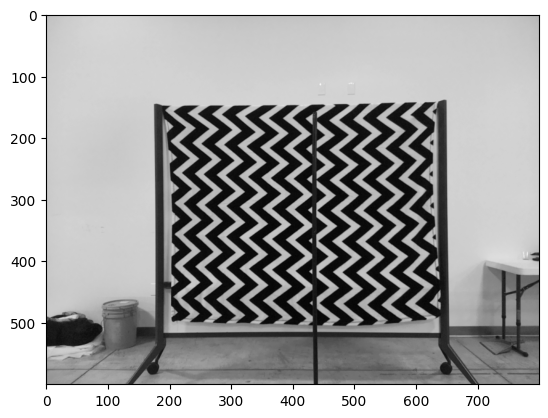
\includegraphics[width=\textwidth]{sections/discussion/zigzag-left-failure-4.png}
            \caption{Left camera image with a single test object.}
            \label{fig:zigzag-2obj-compare:left-single}
        \end{subfigure}
        \hfill
        \begin{subfigure}[b]{0.45\textwidth}
            \centering
            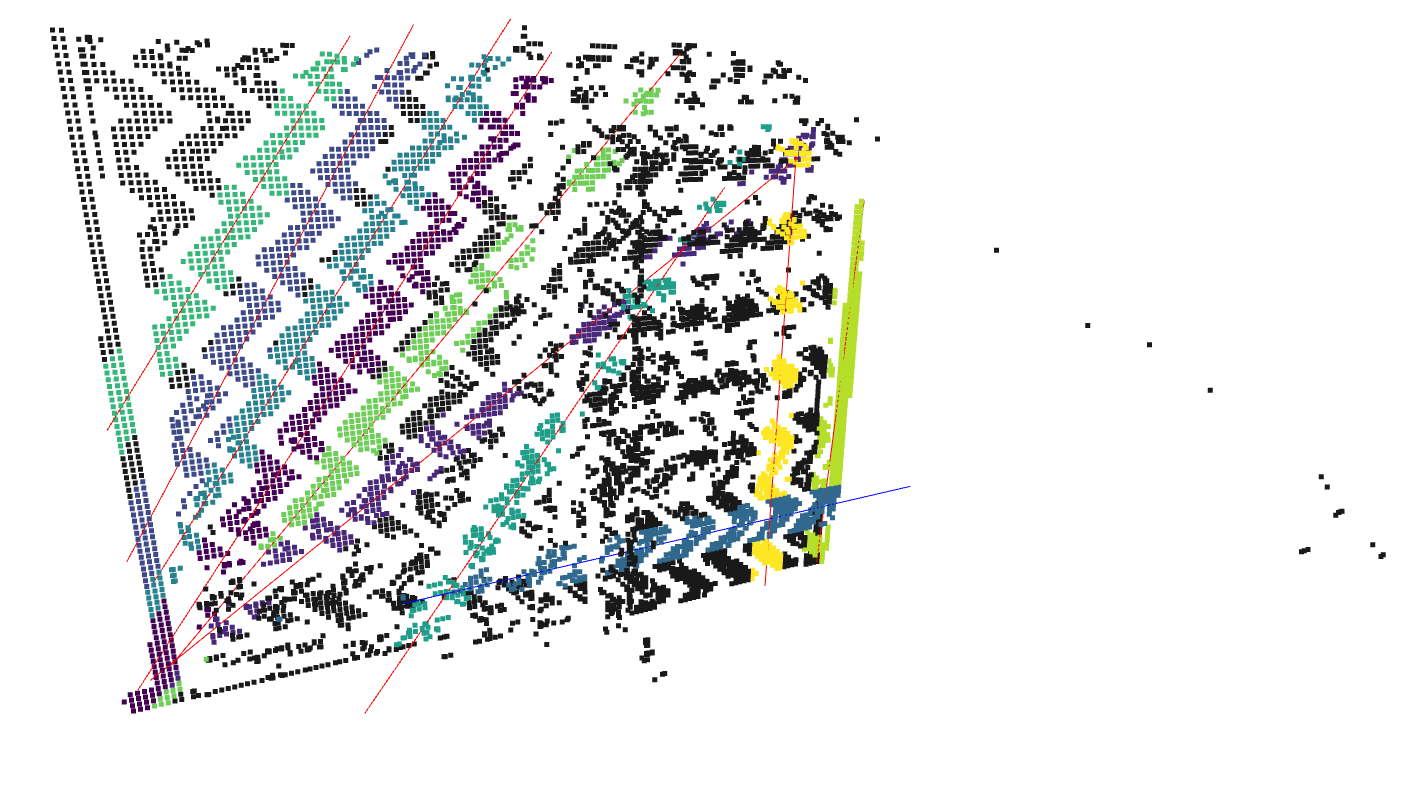
\includegraphics[width=\textwidth]{sections/discussion/zigzag-ptcld-failure-4.png}
            \caption{Point cloud generated from \ref{fig:zigzag-2obj-compare:left-single}, 
                in which the test object has not been detected as a candidate.}
            \label{fig:zigzag-2obj-compare:ptcld-single}
        \end{subfigure}
    \end{subfigure}
    \vfill
    % Generated from "C:\\Users\\wyatt\\Documents\\GVSU\\Thesis\\august_test_data\\idc_sept_5\\blanket_2_obj\\pvc_2000_0_0_0_bin_18"
    \begin{subfigure}[b]{\textwidth}
        \begin{subfigure}[b]{0.45\textwidth}
            \centering
            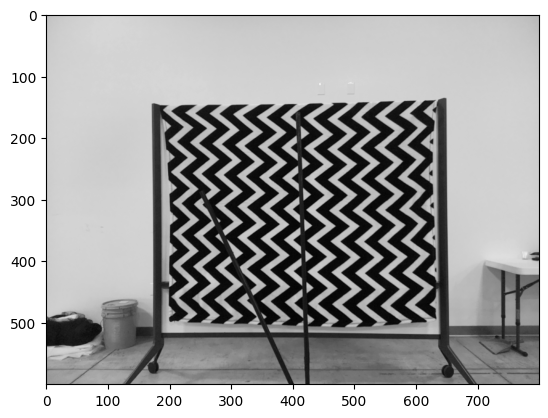
\includegraphics[width=\textwidth]{sections/discussion/zigzag-left-2-obj.png}
            \caption{Left camera image with a single test object.}
            \label{fig:zigzag-2obj-compare:left-double}
        \end{subfigure}
        \hfill
        \begin{subfigure}[b]{0.45\textwidth}
            \centering
            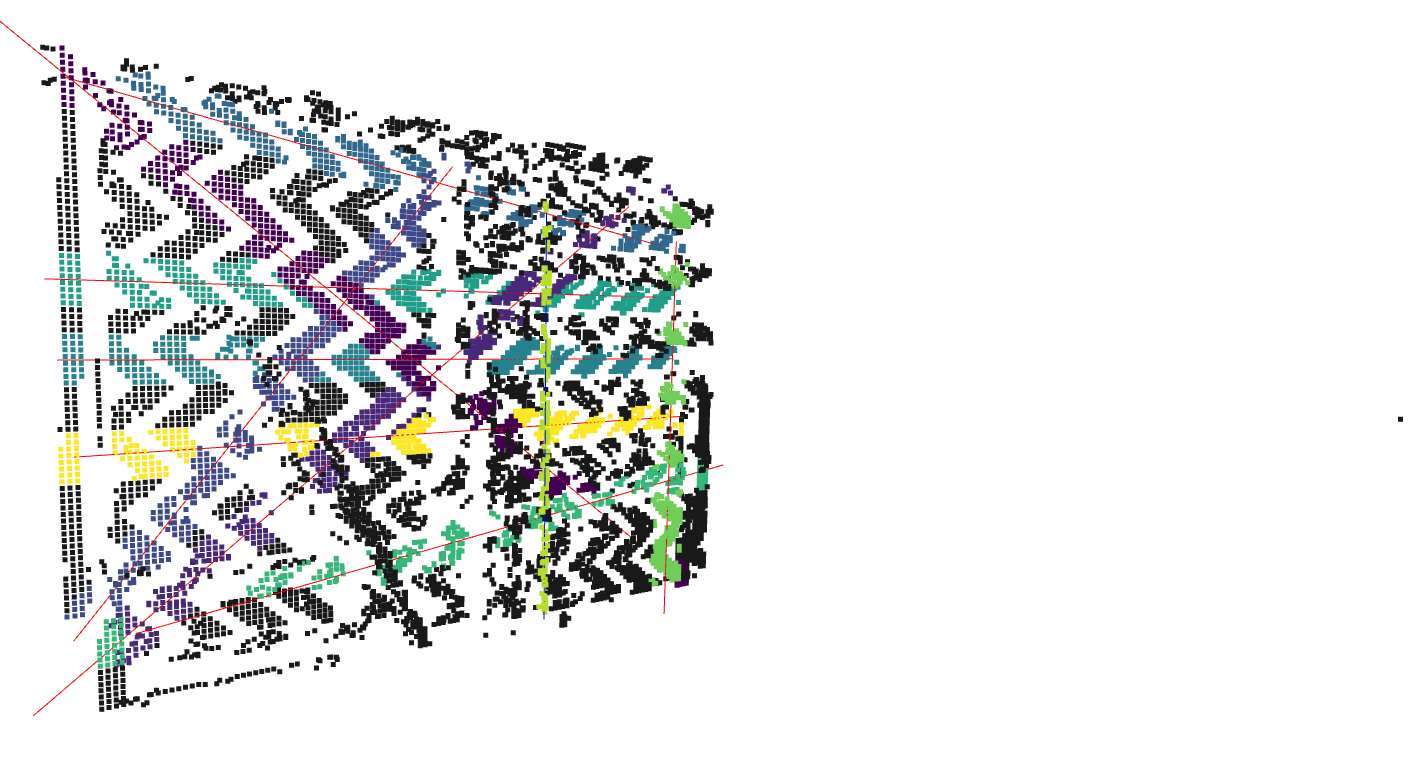
\includegraphics[width=\textwidth]{sections/discussion/zigzag-ptcld-2-obj.png}
            \caption{Point cloud generated from \ref{fig:zigzag-2obj-compare:left-double}, 
                in which the test object has not been detected as a candidate.}
            \label{fig:zigzag-2obj-compare:ptcld-double}
        \end{subfigure}
    \end{subfigure}
    \caption{Sample data from a test with a single object (\ref{fig:zigzag-2obj-compare:left-single} and \ref{fig:zigzag-2obj-compare:ptcld-single})
    in which the object was not correctly detected, and with two objects (\ref{fig:zigzag-2obj-compare:left-double} and \ref{fig:zigzag-2obj-compare:ptcld-double})
    in which the object was correctly detected. Note in \ref{fig:zigzag-2obj-compare:ptcld-double} how the test object is correctly detected, shown as the light green
    points vertically arranged in the center of the point cloud, and the second object is not detected as a candidate line.}
\end{figure}
    
\end{doublespace}


\section{References}
\printbibliography[heading=none]


\begin{appendices}
    \section{Grasper Device OpenSCAD Code}
    \label{app:grasper-scad}
    \inputminted[linenos, frame=lines, breaklines]{c}{"C:/Users/wyatt/Documents/GVSU/Thesis/design/grasper5/clasp.scad"}

    \section{Schematics}
    \label{app:schematics}

    \subsection{CPU Module and Camera Interface}
    \pagebreak
    \begin{sidewaysfigure}[p]
        \centering
        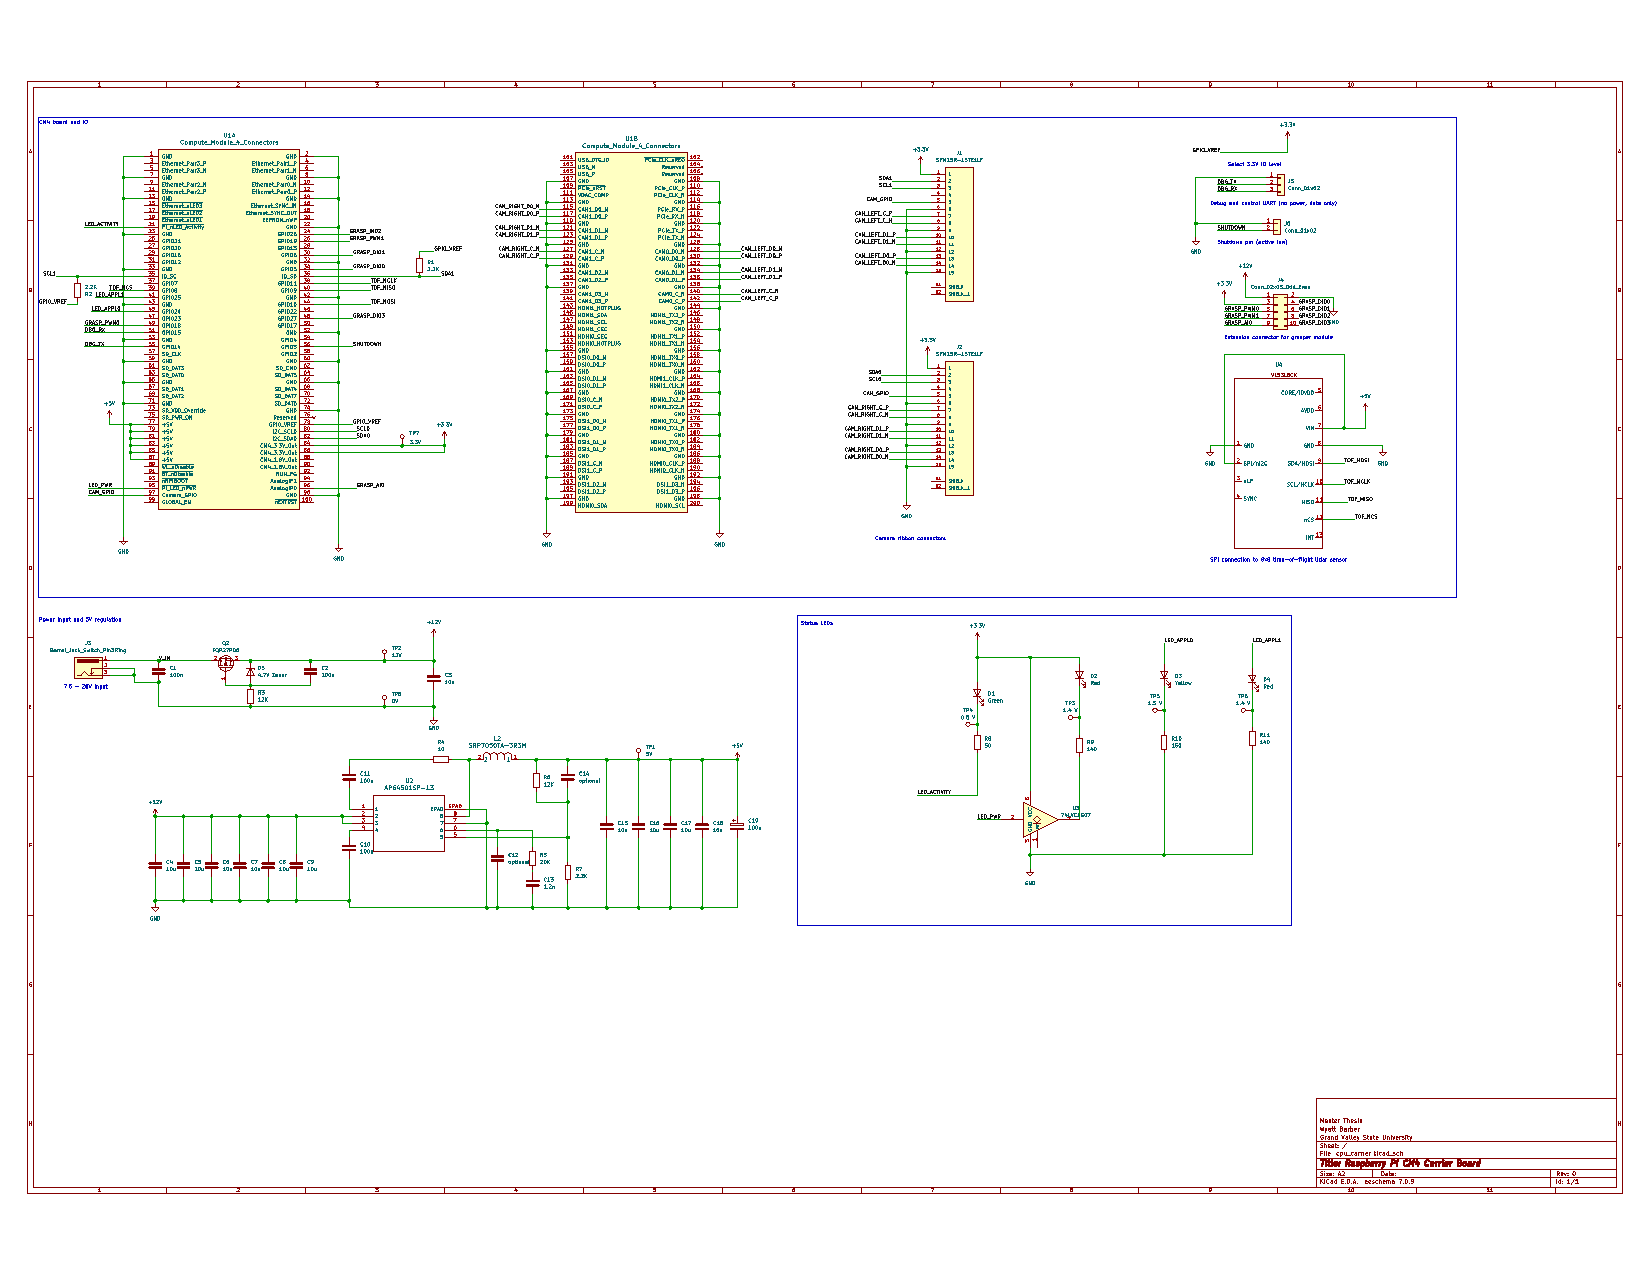
\includegraphics[width=\textwidth]{appendices/cpu-carrier.pdf}
        \caption{Carrier board and camera interface for the CPU. At center-right is J4, the 10-pin 
        interface to the controller in Fig. \ref{fig:clasp-ctl}, as well as debug interfaces. J1 and J2
        are the ribbon connectors for the MIPI CSI interface to the left and right camera. U4 is a time-of-flight
        lidar sensor that was tested but ultimately not used due to poor performance in sunlight. U1 is the CPU,
        and across the bottom of the schematic are power supply components.}
        \label{fig:cpu-module}
    \end{sidewaysfigure}
    \FloatBarrier


    \subsection{Servo Controller}
 
    \begin{sidewaysfigure}[p]
        \centering
        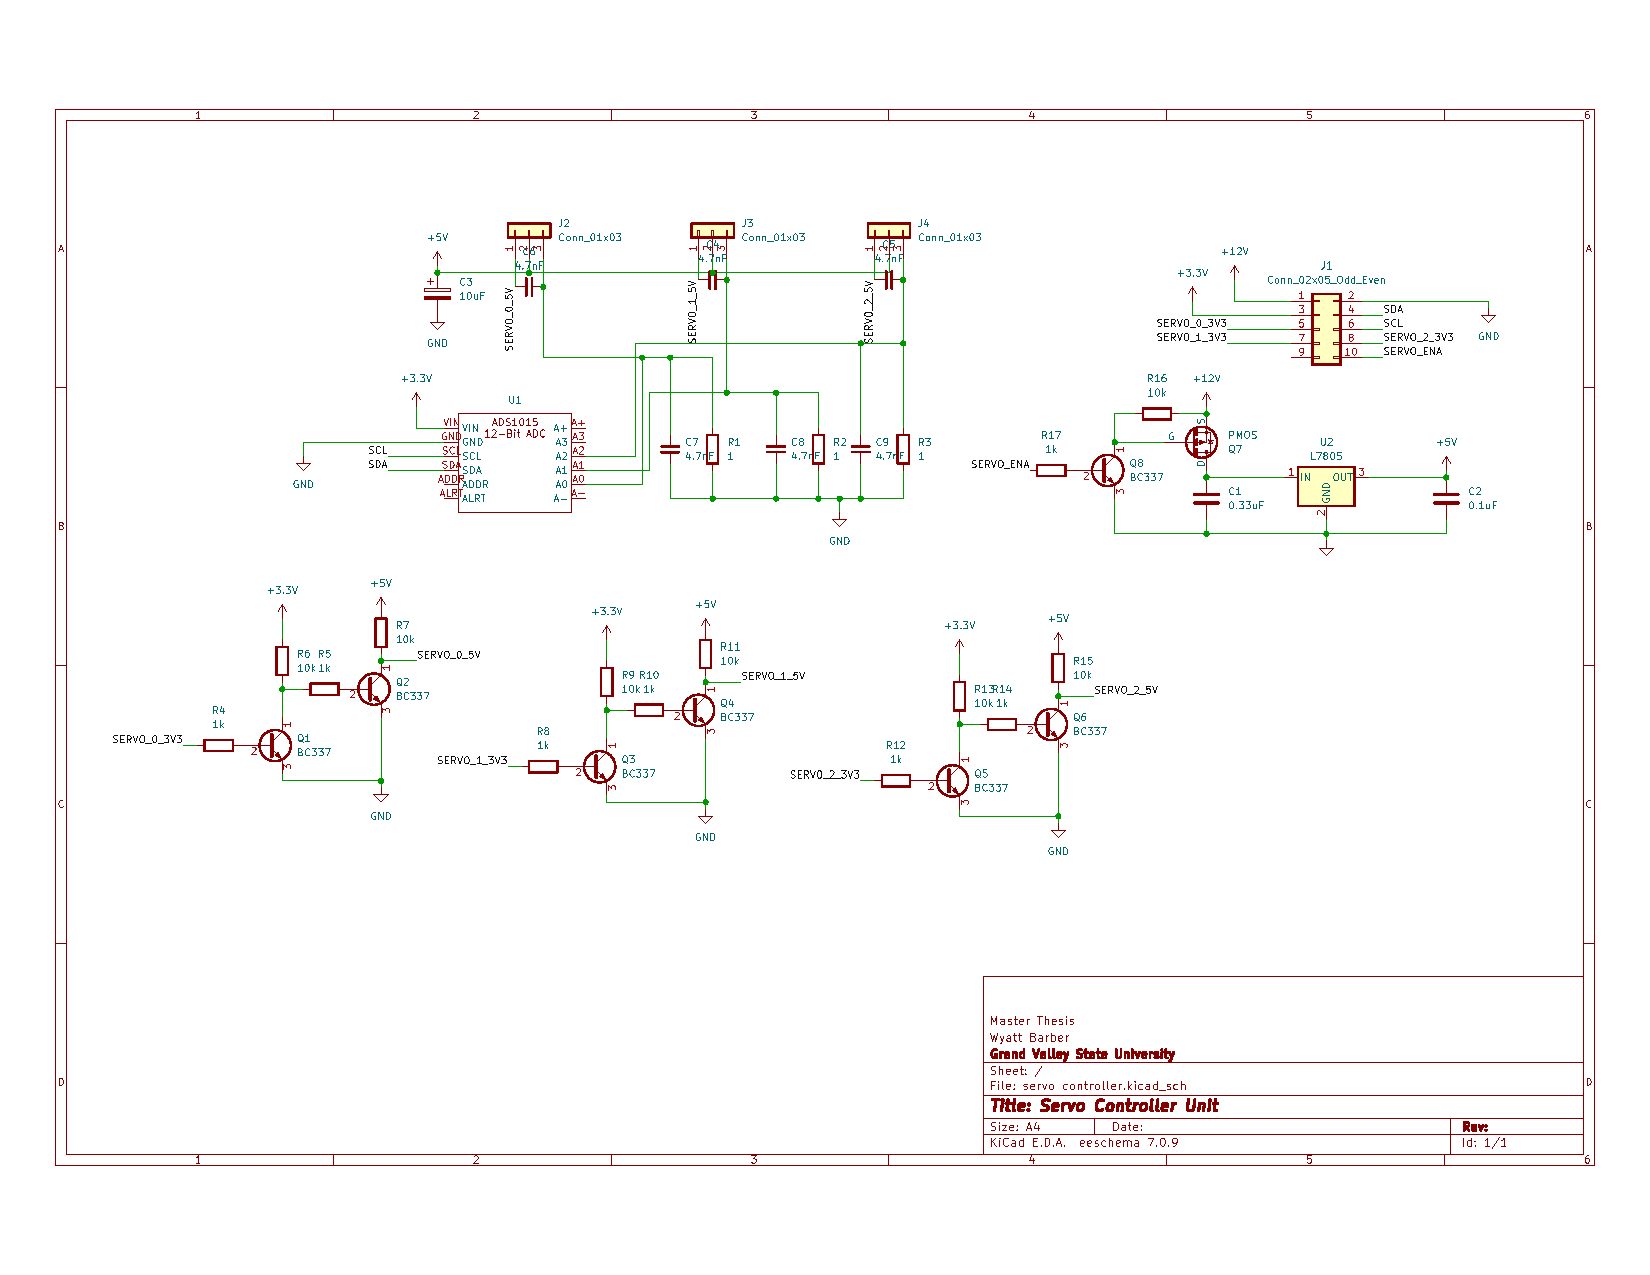
\includegraphics[width=\textwidth]{appendices/grasper-ctl.pdf}
        \caption{Servo control module used for this grasper design, consisting of a 5V regulator
        that can be enabled or disabled digitally, three level shifters for servo PWM signals,
        and an Adafruit ADS1015 analog-digital converter for current measurement.}
        \label{fig:clasp-ctl}
    \end{sidewaysfigure}
    \FloatBarrier

    \section{Main Program Code}
    \label{app:main-code}

    The main program that runs on the Raspberry Pi for image processing and grasper 
    control is too large to insert in an appendix page. For the time being the GitHub link
    below is included until a better means to distribute the program source with the thesis 
    is determined.

    \url{https://github.com/wyattbarber/PerchDetector}    

    \section{Stereo Calibration Script}
    \label{app:cal-code}

    Primary calibration script, exported from a Jupyter notebook.

    \inputminted[linenos, frame=lines, breaklines]{python}{"C:/Users/wyatt/Documents/GVSU/Thesis/calibration and tuning/calibration/calibration export.py"}

    Contents of \texttt{calibration.py}, containing the source for the calibration helper classes.

    \inputminted[linenos, frame=lines, breaklines]{python}{"C:/Users/wyatt/Documents/GVSU/Thesis/calibration and tuning/calibration/calibration.py"}


    \section{Detection Data Collection Script}
    \label{app:data-coll-code}

    \inputminted[linenos, frame=lines, breaklines]{python}{"C:/Users/wyatt/Documents/GVSU/Thesis/PerchDetector/datacollector.py"}

    
    \section{Detection Results Labelling Script}
    \label{app:label-code}

    \inputminted[linenos, frame=lines, breaklines]{python}{"C:/Users/wyatt/Documents/GVSU/Thesis/august_test_data/passfail.py"}

    \section{Simulation Retest Script}
    \label{app:retest-code}

    \inputminted[linenos, frame=lines, breaklines]{python}{"C:/Users/wyatt/Documents/GVSU/Thesis/PerchDetector/sim-retest.py"}

\end{appendices}


%\section{Submission Agreement}


\end{document}